\documentclass[]{article}
\usepackage{graphicx}
\usepackage{subcaption}
\usepackage[table]{xcolor}


%opening
\title{Multi-Phase Steel Micro-structure Segmentation using UNet: Generalization and Magnification Independence Analysis}
\author{[Early Draft]}

\begin{document}

\maketitle

\begin{abstract}
	
The micro-structures of advanced high-strength steel, including constituents such as Martensite, Ferrite, and Bainite, provide crucial insights into the steel's physical properties, but while their manual examination is laborious and prone to subjective bias the other alternatives are cost-prohibitive. Our proposed methodology involves the use of a UNet model to perform image segmentation of steel microstructures, automating the traditionally manual analysis process. This model requires a minimal amount of annotated micrographic images for training, yet it demonstrates excellent performance in segmenting steel microstructures. Importantly, our approach tries to maintain its accuracy across different magnifications and various types of steel, highlighting its versatility and generalizability. This paper contributes to the advancement of industrial processes by offering a scalable, efficient, and objective solution for the characterization of microstructures, significantly improving the metallographic segmentation process in the steel industry.

\end{abstract}

\section{Introduction}

The advent of Artificial Intelligence (AI) has brought about transformative changes across various sectors, including manufacturing processes \cite{russel2010}. AI systems, by encapsulating significant knowledge into models, have become an indispensable component of the Industry 4.0 revolution \cite{lasi2014industry}. In this scenario, the segmentation of metallographic images is pivotal for understanding material characteristics and refining manufacturing procedures, thereby enhancing product quality assessment and fostering the creation of new products \cite{gonzalez2008digital, cv_algandapp}.

Among the various applications in industrial manufacturing, our focus is on the segmentation of metallographic images. Image segmentation, a fundamental problem in computer vision, involves dividing an image into distinct regions based on specific criteria \cite{HARALICK1985100}. This problem has been extensively studied and finds applications in numerous domains, including medical image analysis \cite{Litjens_2017, shen2017}, autonomous driving \cite{chen2017deeplab}, and robotics \cite{garciagarcia2017review}.

Transformation-induced-plasticity (TRIP) effect, is a material phenomenon that occurs in multi-phase microstructures of steel plates. The TRIP effect involves the transformation of retained austenite to martensite during plastic deformation, leading to a significant increase in the work-hardening rate \cite{tripSteels}. This transformation strengthens the neck region, delaying further deformation and enhancing the strength-ductility balance \cite{ALLAIN2004158}. Harnessing the TRIP effect in advanced high-strength steels (AHSS) has emerged as a significant strategy for the steel and automotive industries to maintain high strength and safety properties, while also addressing critical environmental concerns such as fuel consumption and air pollution \cite{BOUAZIZ2011141}. So it becomes essential to find the proper structures of the parts that underwent TRIP effect to access the quality of the produced AHSS. One of the ways to finding the structures in the steel to use obtain images using a Scanning Electron Microscope (SEM) and then generate corresponding labels using methods like Electron Backscatter Diffraction (EBSD). Despite its effectiveness, relying solely on EBSD for routine quality assessment presents several challenges. First, EBSD is not only time-consuming and labor-intensive, but it is also cost-prohibitive for large-scale or frequent analysis. Moreover, while EBSD provides detailed crystallographic information, its resolution is often lower compared to SEM, thus limiting its utility for fine-detail microstructural analysis. Given these challenges, there is a compelling need for alternative, more efficient methods for microstructure characterization. This is where AI-driven image segmentation, specifically using the UNet model, can offer significant advantages. UNet has been widely successful in various domains for its ability to yield precise segmentation, even with fewer training images. Its architecture is particularly suited for biomedical image segmentation, and we extend its application for the segmentation of SEM images of steel microstructures.

However, the segmentation of microscopic steel images is a challenging task due to the intricate nature of steel microstructures and the similarity in appearance among different components when observed under varying magnifications. Unlike general image segmentation problems where objects have distinct boundaries, the components in steel microstructures often exhibit subtle differences and complex structures that require careful analysis for accurate segmentation \cite{NIPS2012_imagenet}. Steel microstructures contain critical information about the mechanical properties and quality of the material, making it essential to accurately separate and identify the different components. This level of detail and precision is particularly crucial in applications such as additive manufacturing, quantitative analysis, and quality control.

Despite the significance of steel image segmentation, there is a scarcity of research specifically addressing this challenge. The existing literature in the field of metallographic segmentation predominantly focuses on limited datasets, where the models are trained and tested on the same set of data, limiting their generalizability. Moreover, previous methods often fail to capture the fine-detailed microstructures, impeding their practical utility in real-world applications \cite{LeCun2015, GoodBengCour16}.

In this study, we propose a scalable metallographic segmentation solution that leverages deep learning techniques and incorporates different augmentation strategies to overcome the limitations of traditional methods. By training on a known set of inputs and testing on diverse magnified images and steel types, our approach aims to provide accurate and detailed segmentation results, advancing the field of steel image analysis and supporting industrial applications in a more robust and comprehensive manner. Our proposed approach has several advantages. First, it substantially reduces the time and cost associated with microstructure characterization, as compared to EBSD. Second, it allows for high-resolution, detailed segmentation of microstructures, given the superior resolution of SEM images. Lastly, it enables large-scale, routine analysis of steel microstructures, thus facilitating regular quality assessment and control in industrial applications. EBSD still remains necessary for generating ground truth labels for SEM images and for occasional validation of segmentation results.

The subsequent sections of this paper elaborate on our proposed methodology and present experimental results demonstrating its effectiveness in automating microstructure characterization. Section 2 reviews related works in the domain. Section 3 discusses the characteristics and challenges of microstructure segmentation, as well as the UNet architecture and dataset. Section 4 presents the methodology, including model architecture, augmentations, and training process. Section 5 focuses on experimentation, covering evaluation metrics, experimental setup, and results on both training and inference images. Section 6 provides a detailed discussion and analysis of the experimental results, addressing challenges, limitations, and factors influencing performance variations. Finally, section 7 concludes by summarizing the key findings, emphasizing the importance of accurate microstructure segmentation, and suggesting future research directions.

\section{Related Works}

The application of deep learning techniques, particularly convolutional neural networks (CNNs), has shown promising results in various image segmentation tasks. The UNet architecture, a type of CNN, has been widely used for medical image segmentation due to its ability to capture both local and global context by using a symmetric encoder-decoder structure \cite{cao2021swinunet}.

In the realm of microstructure segmentation, previous studies have explored various methodologies to achieve accurate classification and segmentation results. Velichko et al. proposed a method based on data mining techniques, specifically extracting morphological features and utilizing a feature classification step using Support Vector Machines (SVMs). This approach was applied to cast iron and demonstrated the potential of machine learning in microstructural analysis \cite{sym13071176}. However, this method, while effective for simpler microstructures, may not be as efficient for complex steel microstructures due to the intricate nature and the subtle differences among different components.

Similarly, Pauly et al. adopted a similar approach on a contrasted and etched dataset of steel acquired through SEM and LOM imaging \cite{LAI2009665}. However, the results yielded a relatively low accuracy of 48.89\% in microstructural classification due to the complex nature of substructures and the lack of discriminative features. This highlights the need for a more robust and efficient method for microstructure segmentation.

Durmaz et al. proposed a multidisciplinary deep learning approach that equally considers specimen preparation and imaging \cite{Durmaz2021}. They trained distinct UNet architectures with 30-50 micrographs of different imaging modalities and electron backscatter diffraction-informed annotations. The study focused on the challenging task of lath-bainite segmentation in complex-phase steel, achieving accuracies of 90\% that rival expert segmentations. While this approach has shown promising results, it requires a large number of annotated images for training, which may not always be feasible in practical scenarios.

In contrast to these previous works, our proposed method aims to provide a scalable solution that requires only a small number of annotated images for training. We leverage different augmentation strategies to increase the diversity of our training data, thereby enhancing the robustness and generalizability of our model. Furthermore, our approach is designed to handle different magnified images and steel types, making it more versatile and applicable to a wider range of scenarios.

In summary, while previous studies have made significant contributions to the field of microstructure segmentation, our work aims to address the limitations of these methods by proposing a scalable, efficient, and versatile solution for steel microstructure segmentation.

\section{Background}
This section provides an overview of the key aspects of the semantic segmentation problem in the context of microstructures. It also discusses the dataset utilized in this study and highlights the associated challenges.
\subsection{Characteristics and Challenges of Microstructure Segmentation}
Segmenting microstructures in metallographic images presents a highly challenging task due to the distinctive visual characteristics inherent in these images.

Microstructure segmentation in microscopic steel images is complex due to several factors. Firstly, these images contain high-resolution details that necessitate precise detection and segmentation of fine-grained structures. Furthermore, the inherent variability in textures and shapes within these images adds to the challenge of accurately distinguishing and segmenting different regions. Additionally, imbalanced class distributions, where some components are more prevalent than others, introduce difficulties in achieving accurate segmentation results across all classes. Moreover, the absence of landmark information in these images limits the availability of unique characteristics that could aid in capturing the distinct features of microstructures \cite{LUENGO2022232}.

Due to the heterogenous material properties in these metallographic images, accurately delineating and classifying different regions becomes difficult. Heterogenous properties also heighten the variations in scale and magnification, leading to changes in the appearance and size of the microstructures.

While manual annotation of metallographic images is a labor-intensive and time-consuming, producing EBSD images is cost-prohibitive and not suitable for more frequent analysis. As a result, there is a scarcity of large, labeled datasets specifically tailored for microstructure segmentation \cite{Roberts2019}. This limitation hinders the application of supervised learning methods, which typically require ample training data to achieve optimal performance.

\subsection{Why UNet: An Ideal Choice for Microstructure Segmentation}

The choice of an appropriate model is crucial for achieving accurate results in steel image segmentation. Given the challenges specific to steel microstructure segmentation, we selected the UNet architecture \cite{ronneberger2015unet} for its suitability.

UNet, a convolutional neural network (CNN) architecture, has demonstrated exceptional performance in segmentation tasks, particularly in capturing fine details and handling varying scales of structures. It was originally designed for biomedical image segmentation, where the availability of annotated training data is often limited, and the need for detailed segmentation is high. These characteristics make UNet an ideal choice for the segmentation of steel microstructures.The UNet architecture is characterized by its U-shaped design, which consists of a contracting path to capture context and a symmetric expanding path that allows precise localization. This design enables the model to preserve fine-grained details while capturing global context, making it suitable for steel microstructure segmentation. Another key feature of UNet is the incorporation of skip connections, which allow the fusion of features from multiple scales. This enhances the model's ability to capture intricate details and accurately segment complex structures, a crucial requirement in steel microstructure segmentation.
Furthermore, UNet is designed to work with very few training images and yields more precise segmentations. This is particularly beneficial in our case, where the availability of pixel-wise labels generated through EBSD is limited.

\subsection{Dataset Characteristics and Composition}

The dataset leveraged in our study consists of six E-type steel images captured through a Scanning Electron Microscope (SEM). Due to the minuscule size of the phases in this type of steel, using optical microscopy (OM) for image capture is ineffective. Thus, SEM provides the necessary resolution and detail for effective analysis.

Corresponding to each SEM image, we generated ground truth labels using Electron Backscatter Diffraction (EBSD), providing precise information about the distinct components and phases present within the steel microstructures. In total, the dataset contains images belonging to three different classes, each corresponding to a different phase of the steel microstructure. The labeling colors for each class are as follows:
\begin{itemize}
	\item Orange: Ferrite
	\item Purple: Bainite
	\item Yellow: Martensite
\end{itemize}

The steel used in this study is termed 590DP, which signifies a dual-phase steel with a tensile strength of 590MPa. This kind of steel, also known as gigasteel when the tensile strength reaches 1GPa, is classified as ultra-high-strength steel and is commonly used in automotive applications due to its exceptional strength and formability.

Labeling of the SEM images was accomplished using a superpixel labeling method. Superpixel segmentation groups pixels into larger, coherent superpixels based on similarity in color, texture, and other factors, thus providing a more efficient and accurate labeling process for our dataset. This approach, coupled with the precision of SEM imaging and the detailed phase information from EBSD, ensures the creation of a robust and comprehensive dataset for training and testing our UNet segmentation model.

\begin{figure}[ht]
	\centering
	\begin{subfigure}[b]{0.45\textwidth}
		\centering
		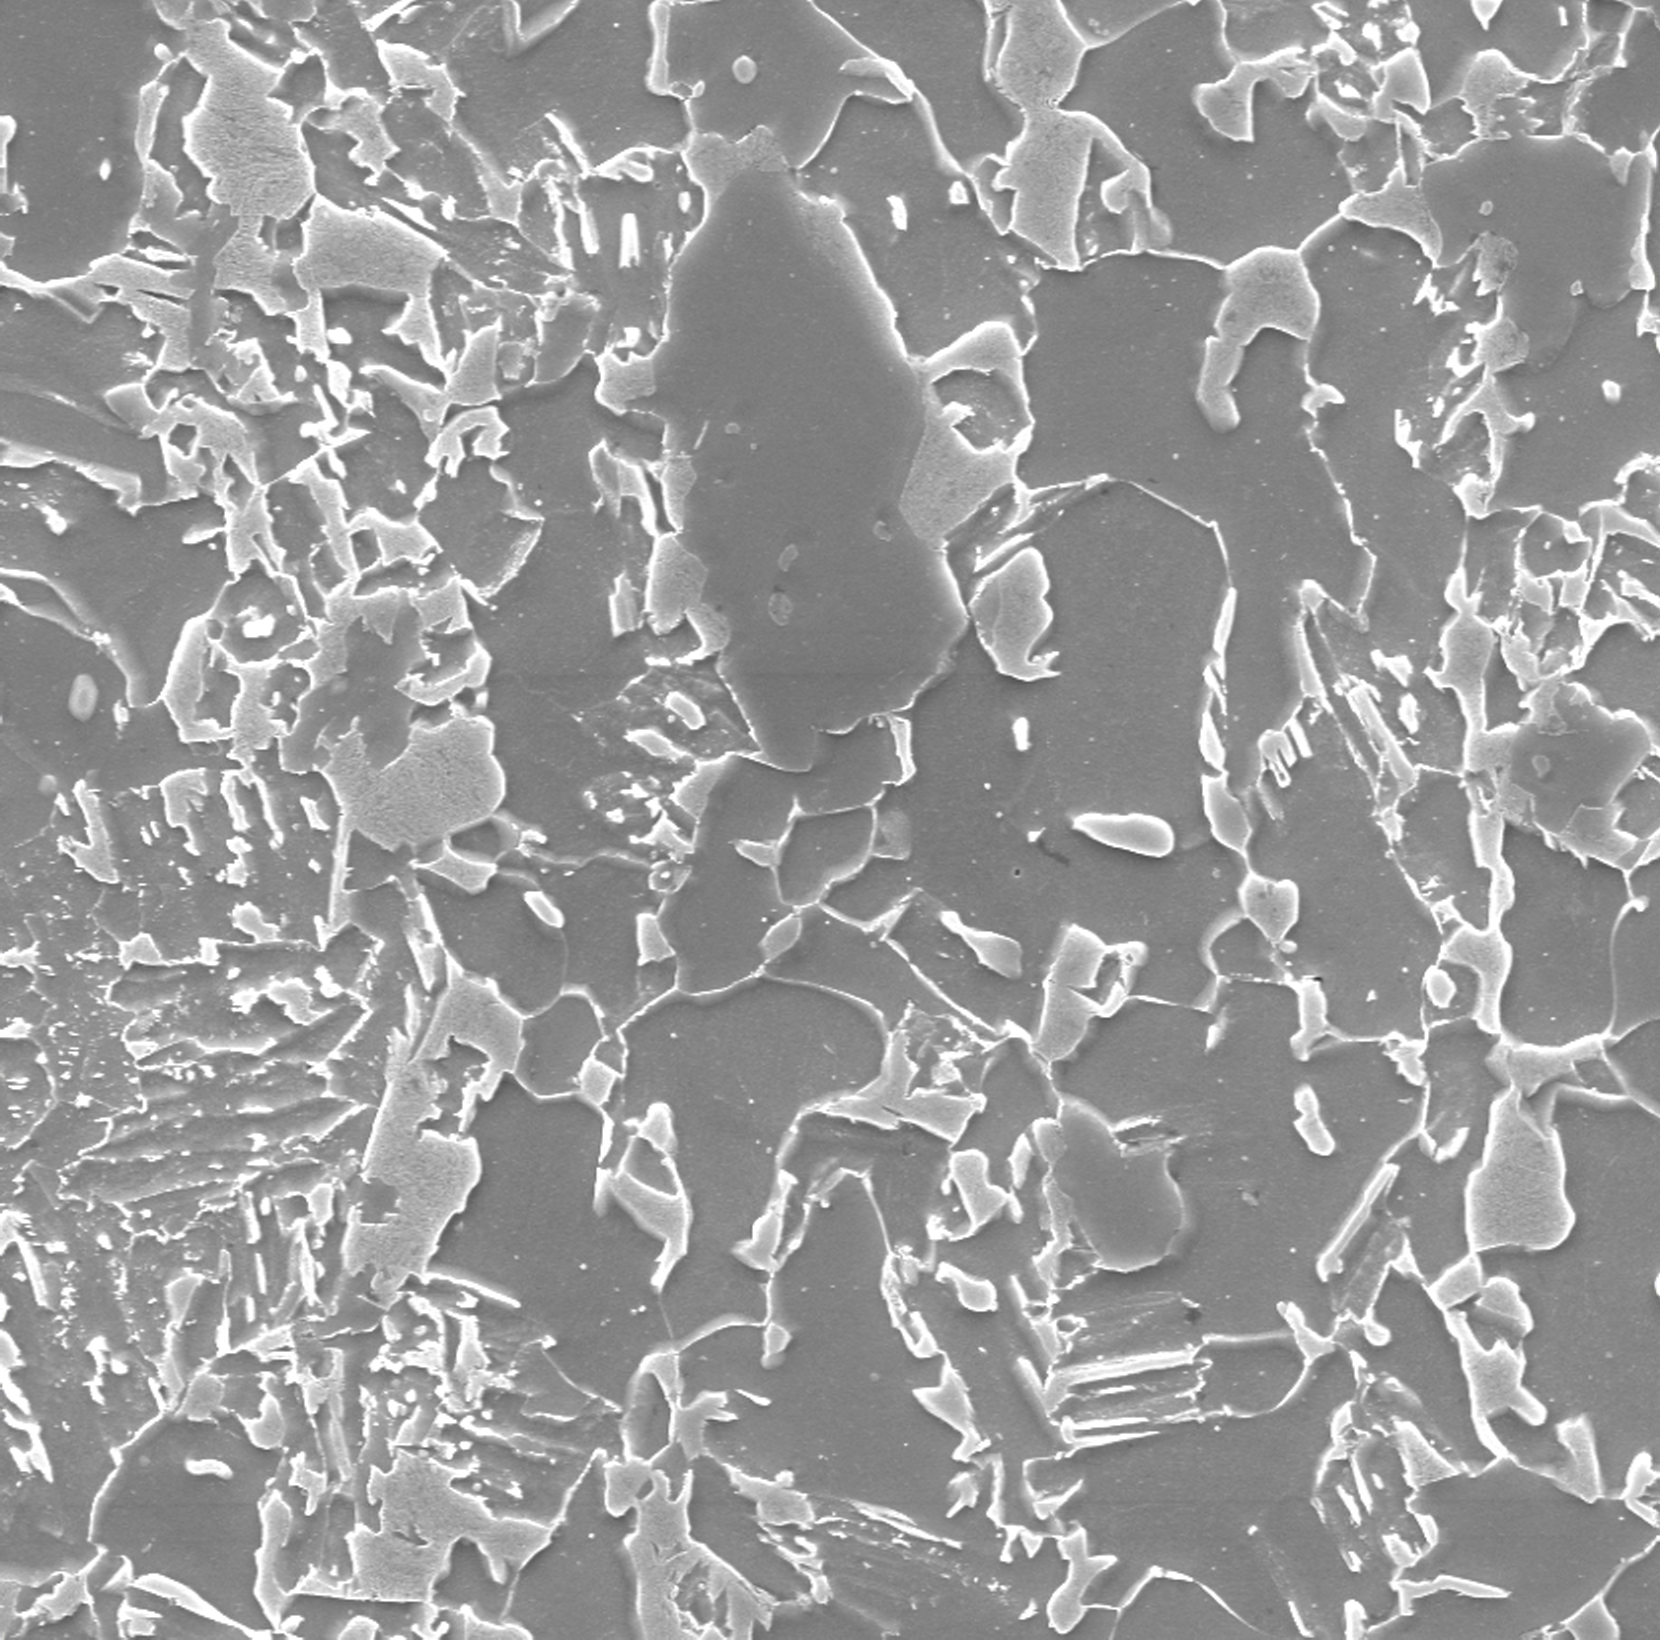
\includegraphics[width=\textwidth]{images/1.png}
		\caption{SEM image}
		\label{fig:image1}
	\end{subfigure}
	\hfill
	\begin{subfigure}[b]{0.45\textwidth}
		\centering
		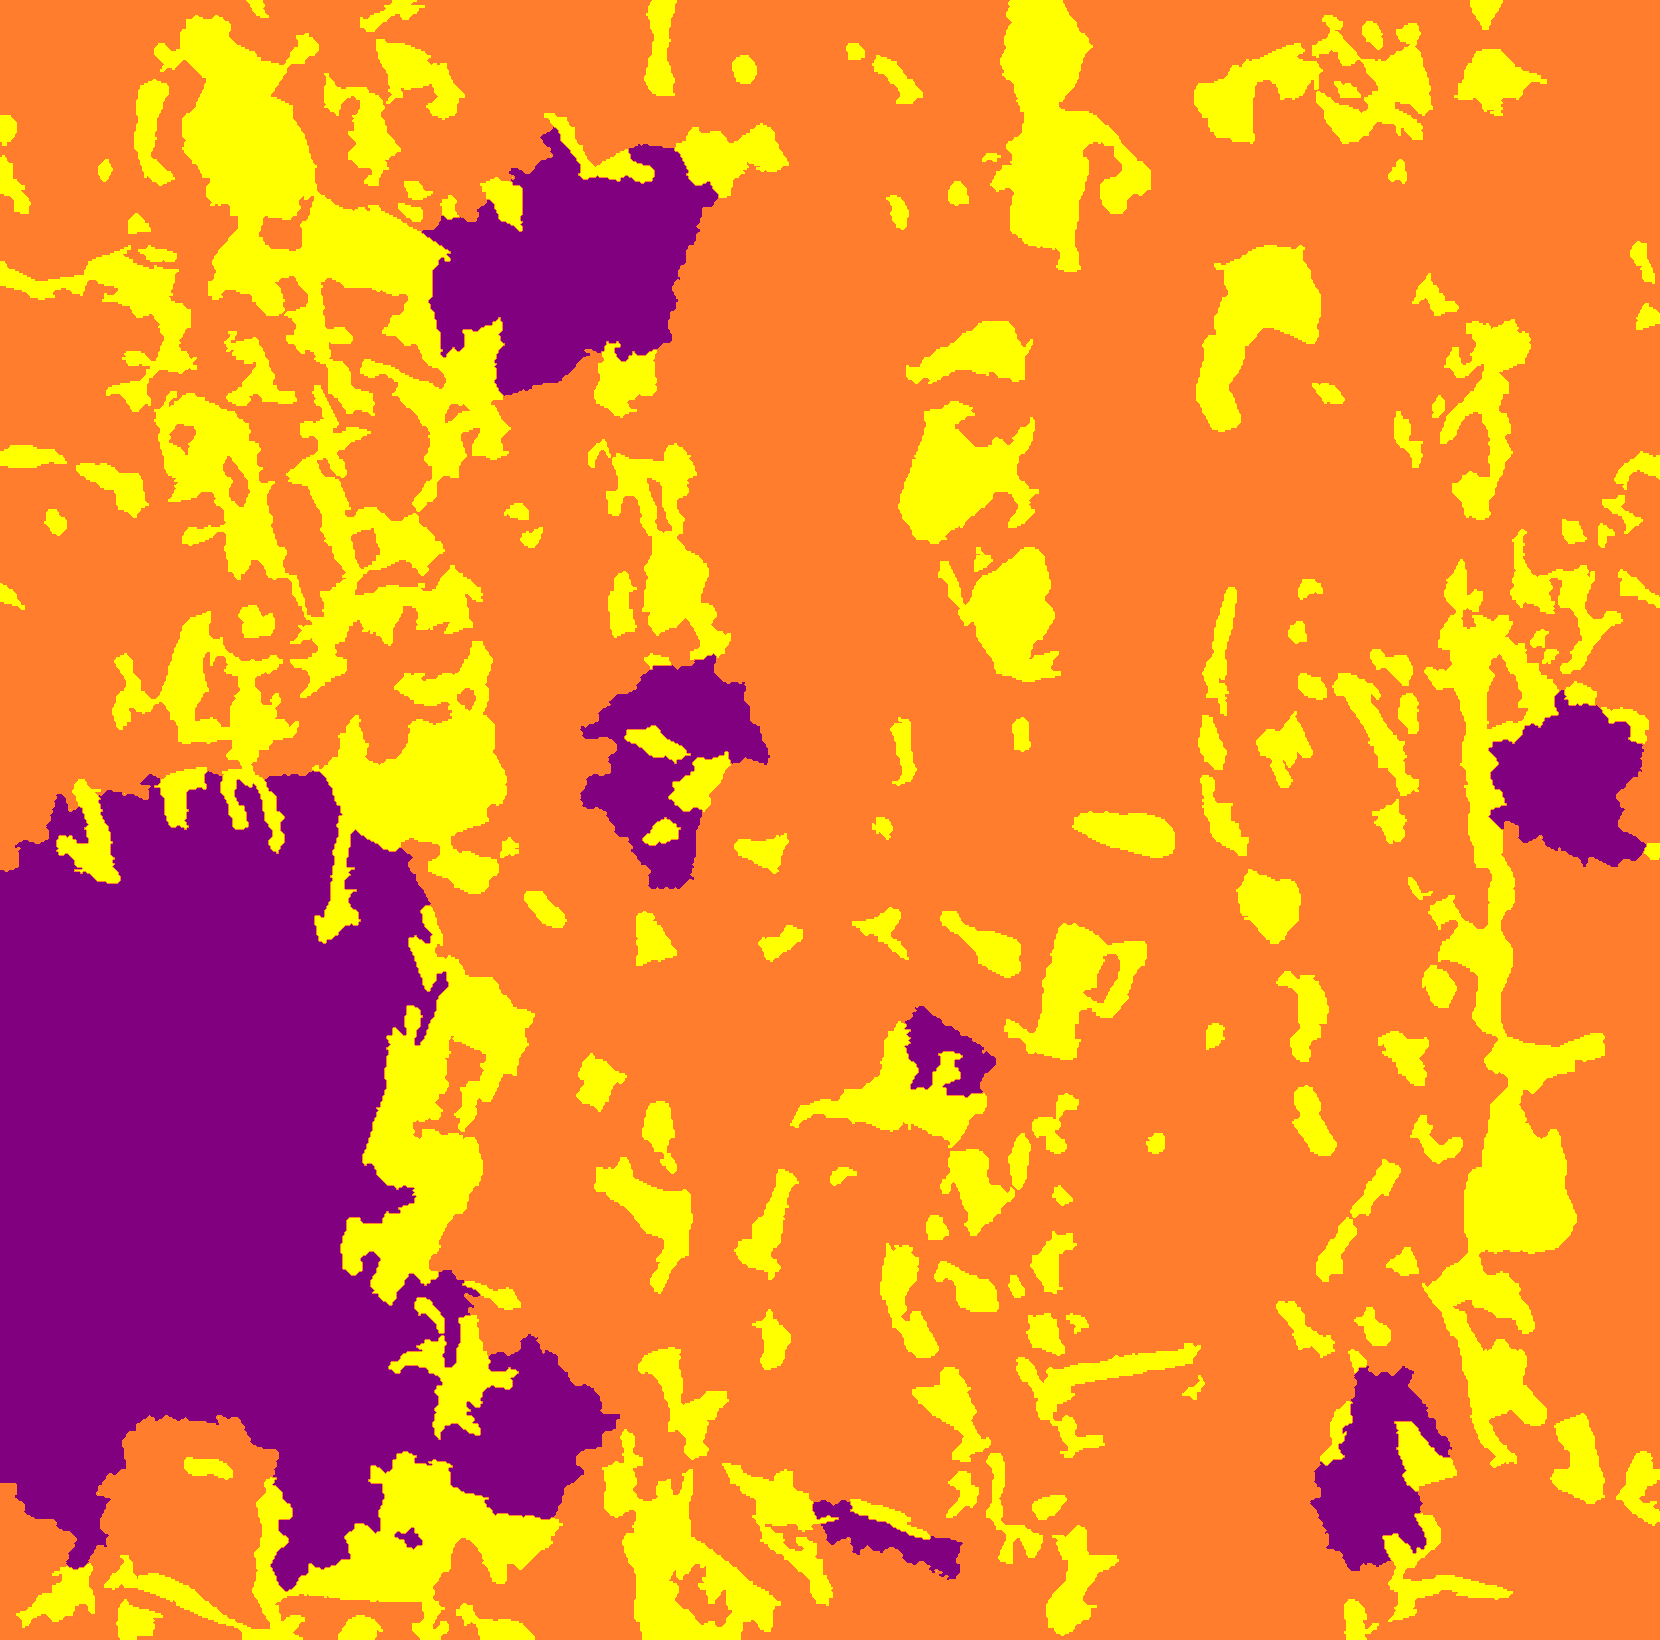
\includegraphics[width=\textwidth]{images/1_label.png}
		\caption{EBSD and Superpixel labeling }
		\label{fig:image2}
	\end{subfigure}
	\caption{x2700 magnified E-type steel image and its corresponding label}
	\label{fig:combined}
\end{figure}


In the training phase of our study, we utilized five out of the six E-type steel images to augment and train the UNet model. The remaining image served as an initial testing ground to validate the model's learning.

To evaluate the model's performance and its ability to generalize, we extended our testing to include steel images magnified at higher magnifications of 3000x and 5000x. The ability to accurately segment images at these higher magnifications is crucial, as it enables the detailed analysis of complex microstructures that are typically observed at these scales.

Furthermore, to test the model's versatility and its effectiveness across various steel types, our testing dataset was expanded to include images of A-type, H2-type, and D3-type steels. These additional steel types have unique microstructural characteristics that pose different challenges to image segmentation. By testing the model across these diverse types of steel, we aim to validate its robustness and its potential for broad applicability in industrial settings.

\begin{figure}[ht]
	\centering
	\begin{subfigure}[b]{0.2\textwidth}
		\centering
		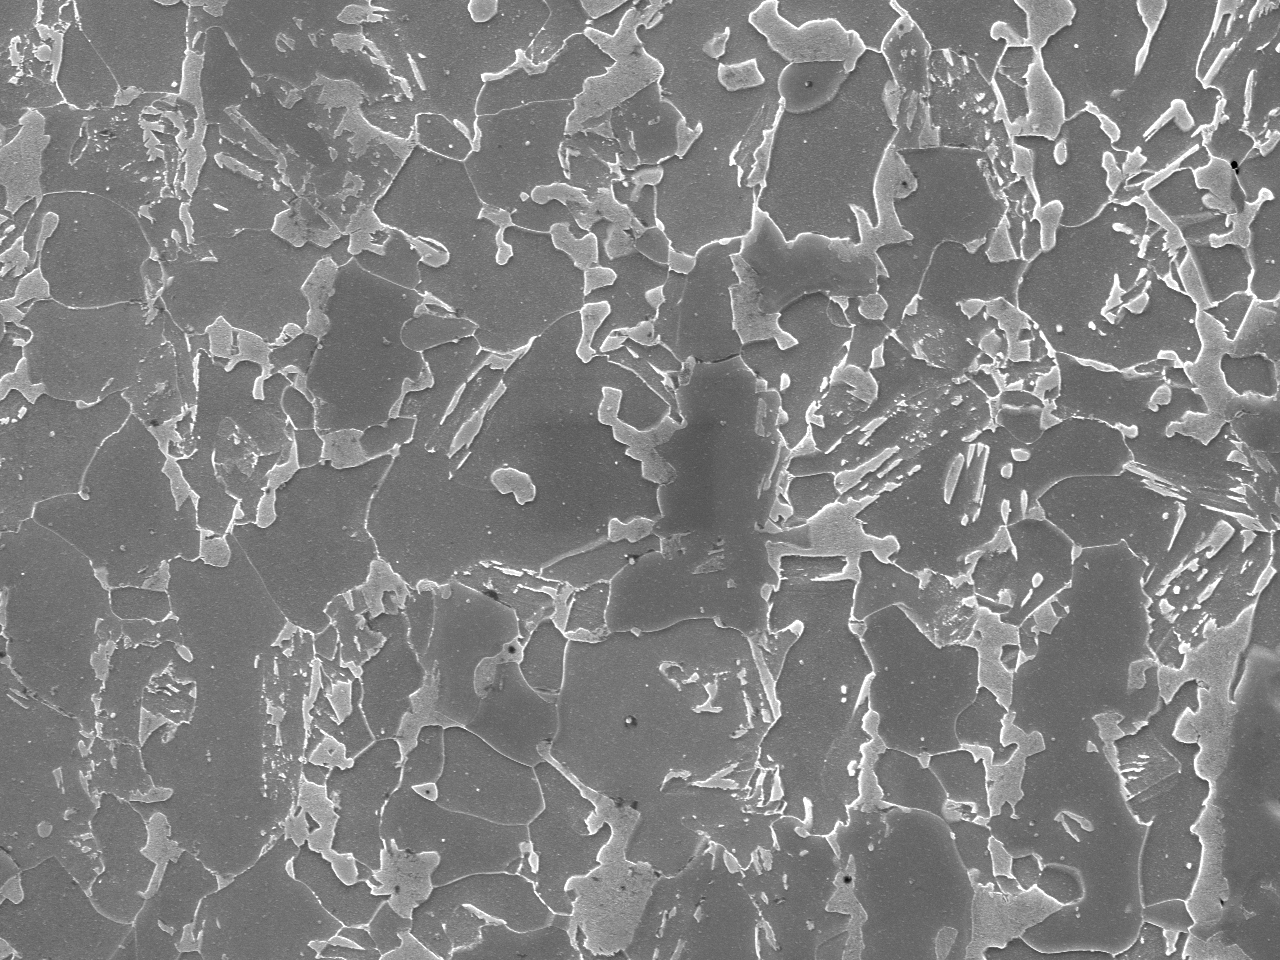
\includegraphics[width=\textwidth]{images/x3000/1.png}
		\caption{x3000 SEM}
		\label{fig:image2.1.1}
	\end{subfigure}
	\begin{subfigure}[b]{0.2\textwidth}
		\centering
		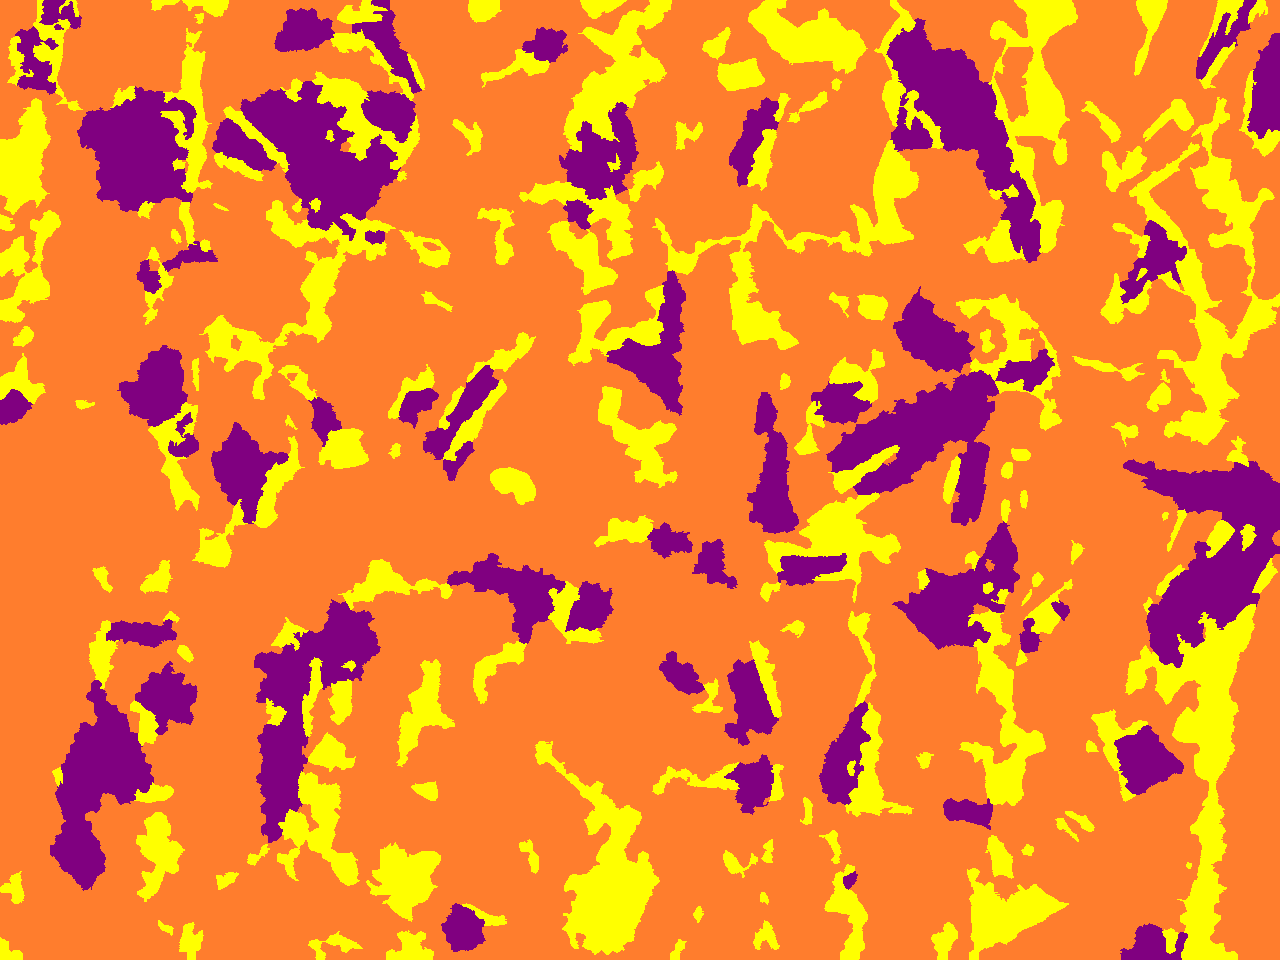
\includegraphics[width=\textwidth]{images/x3000/1_label.png}
		\caption{x3000 label}
		\label{fig:image2.1.2}
	\end{subfigure}
	\hfill
	\begin{subfigure}[b]{0.2\textwidth}
		\centering
		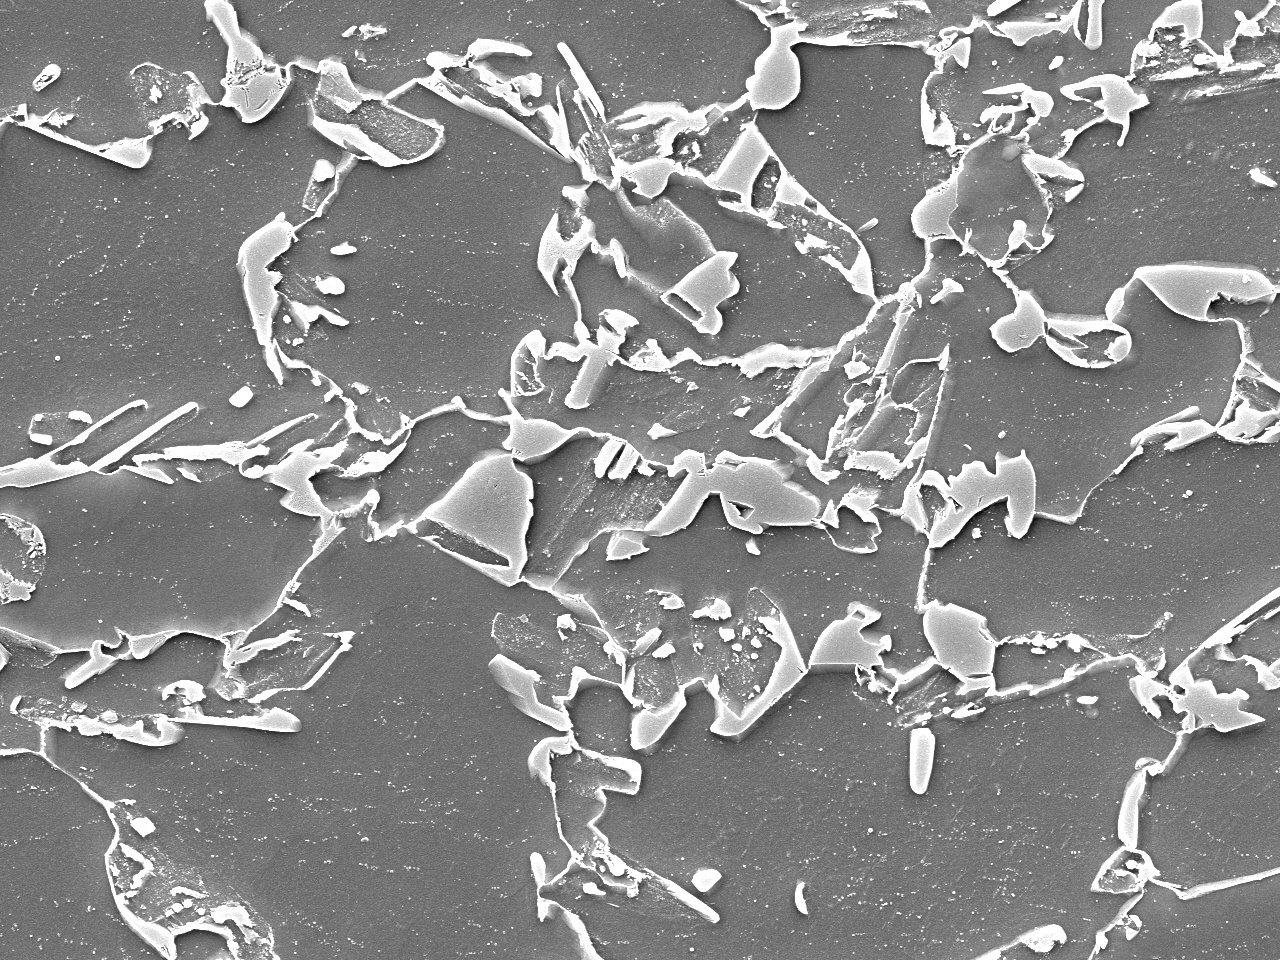
\includegraphics[width=\textwidth]{images/x5000/1.png}
		\caption{x5000 SEM}
		\label{fig:image2.2.1}
	\end{subfigure}
	\begin{subfigure}[b]{0.2\textwidth}
		\centering
		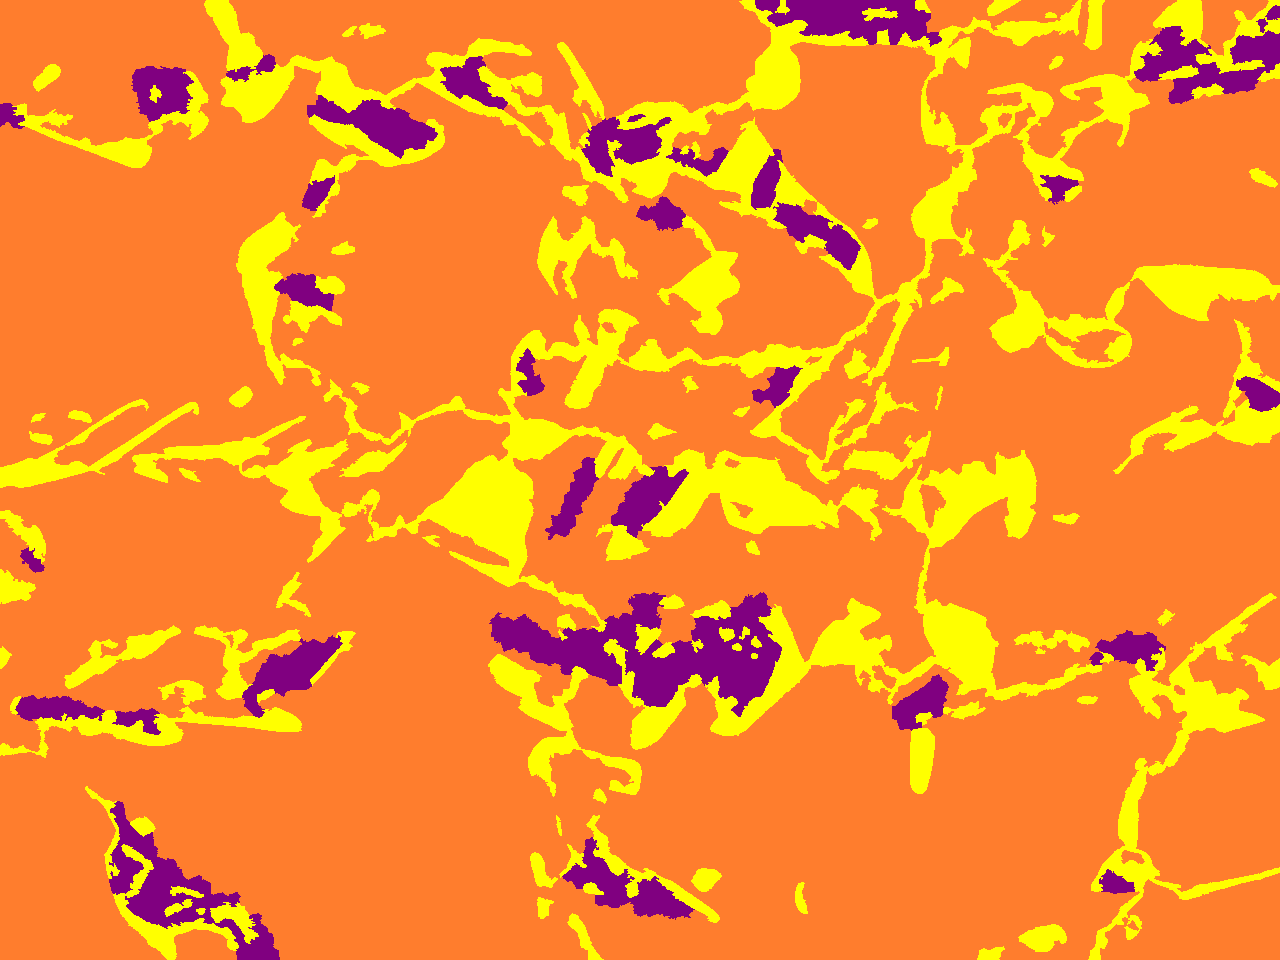
\includegraphics[width=\textwidth]{images/x5000/1_label.png}
		\caption{x5000 label}
		\label{fig:image2.2.2}
	\end{subfigure}
	
	\begin{subfigure}[b]{0.2\textwidth}
		\centering
		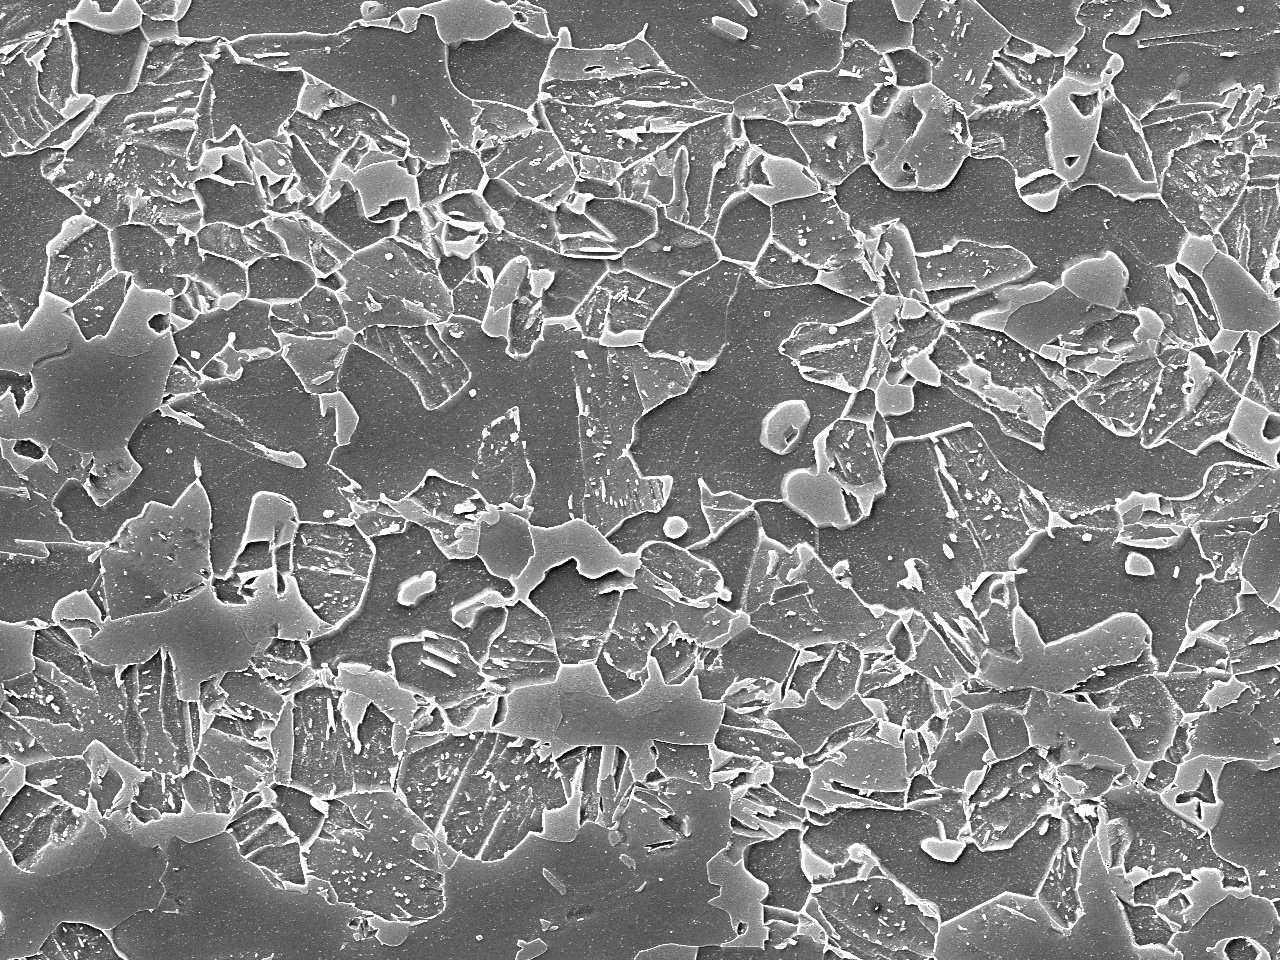
\includegraphics[width=\textwidth]{images/A-type/1.png}
		\caption{A-type SEM}
		\label{fig:image2.3.1}
	\end{subfigure}
	\begin{subfigure}[b]{0.2\textwidth}
		\centering
		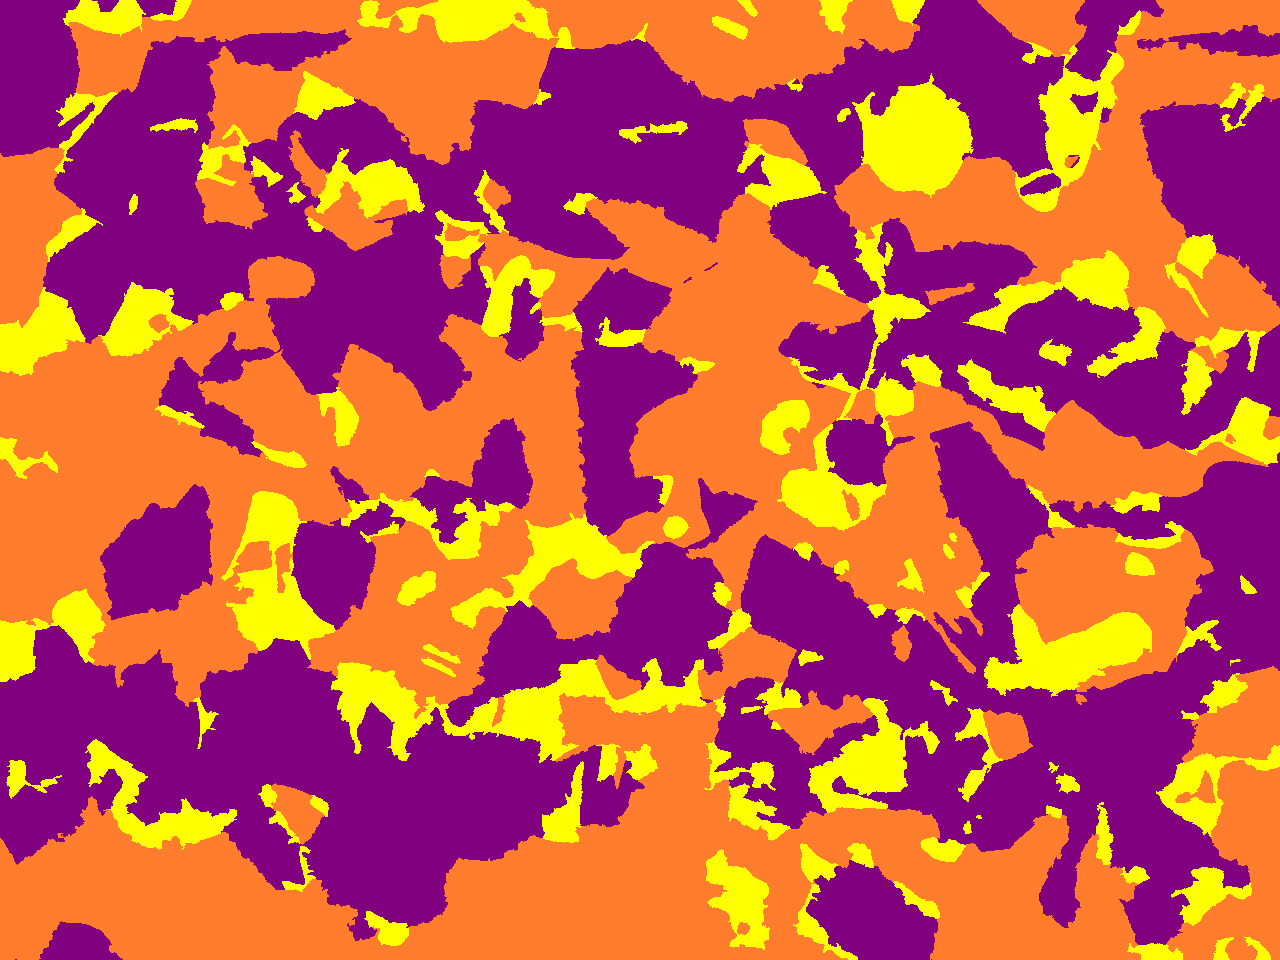
\includegraphics[width=\textwidth]{images/A-type/1_label.png}
		\caption{A-type label}
		\label{fig:image2.3.2}
	\end{subfigure}
	\hfill
	\begin{subfigure}[b]{0.2\textwidth}
		\centering
		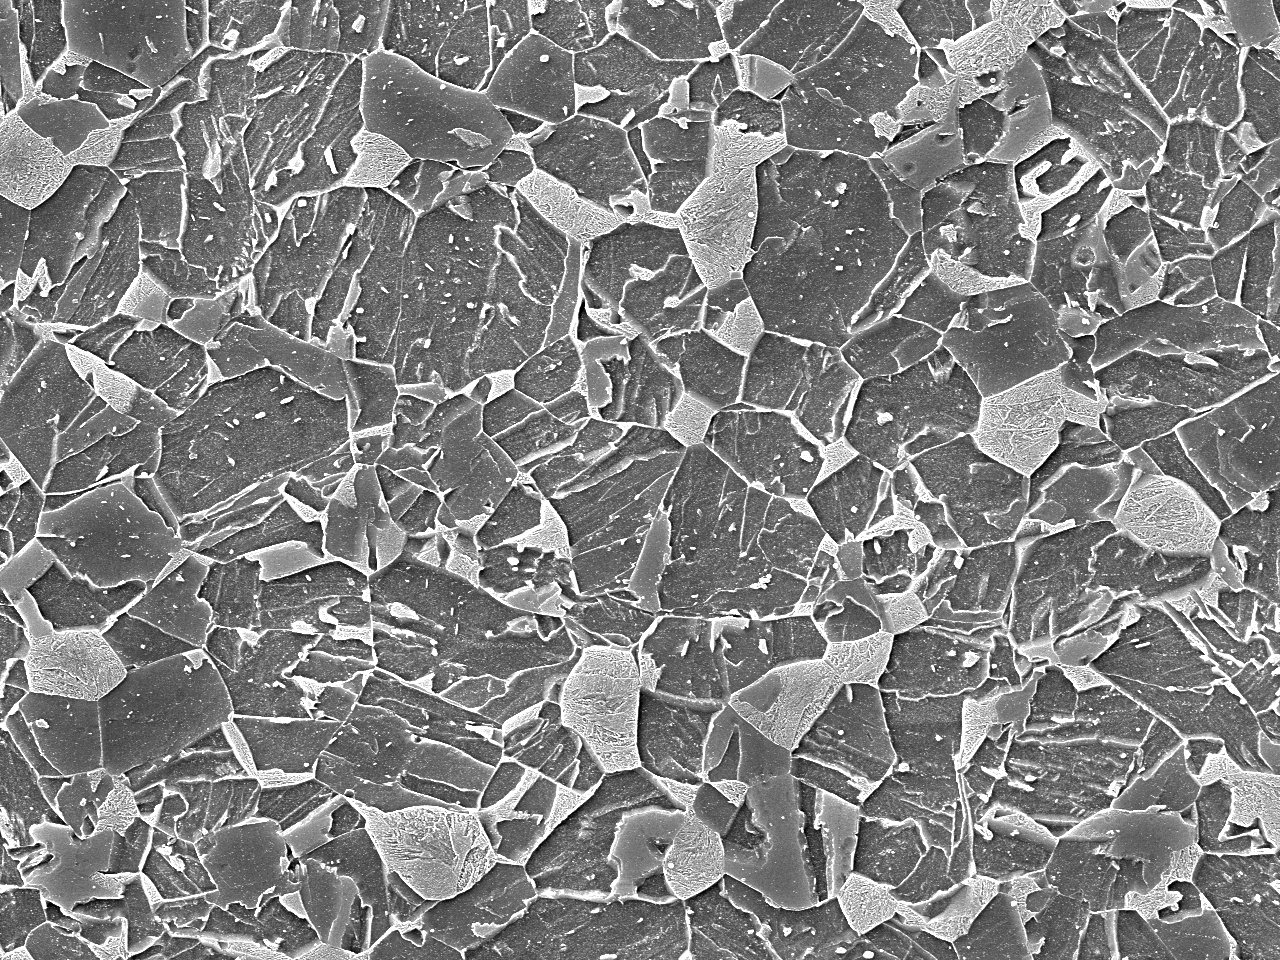
\includegraphics[width=\textwidth]{images/D3-type/1.png}
		\caption{D3-type SEM}
		\label{fig:image2.4.1}
	\end{subfigure}
	\begin{subfigure}[b]{0.2\textwidth}
		\centering
		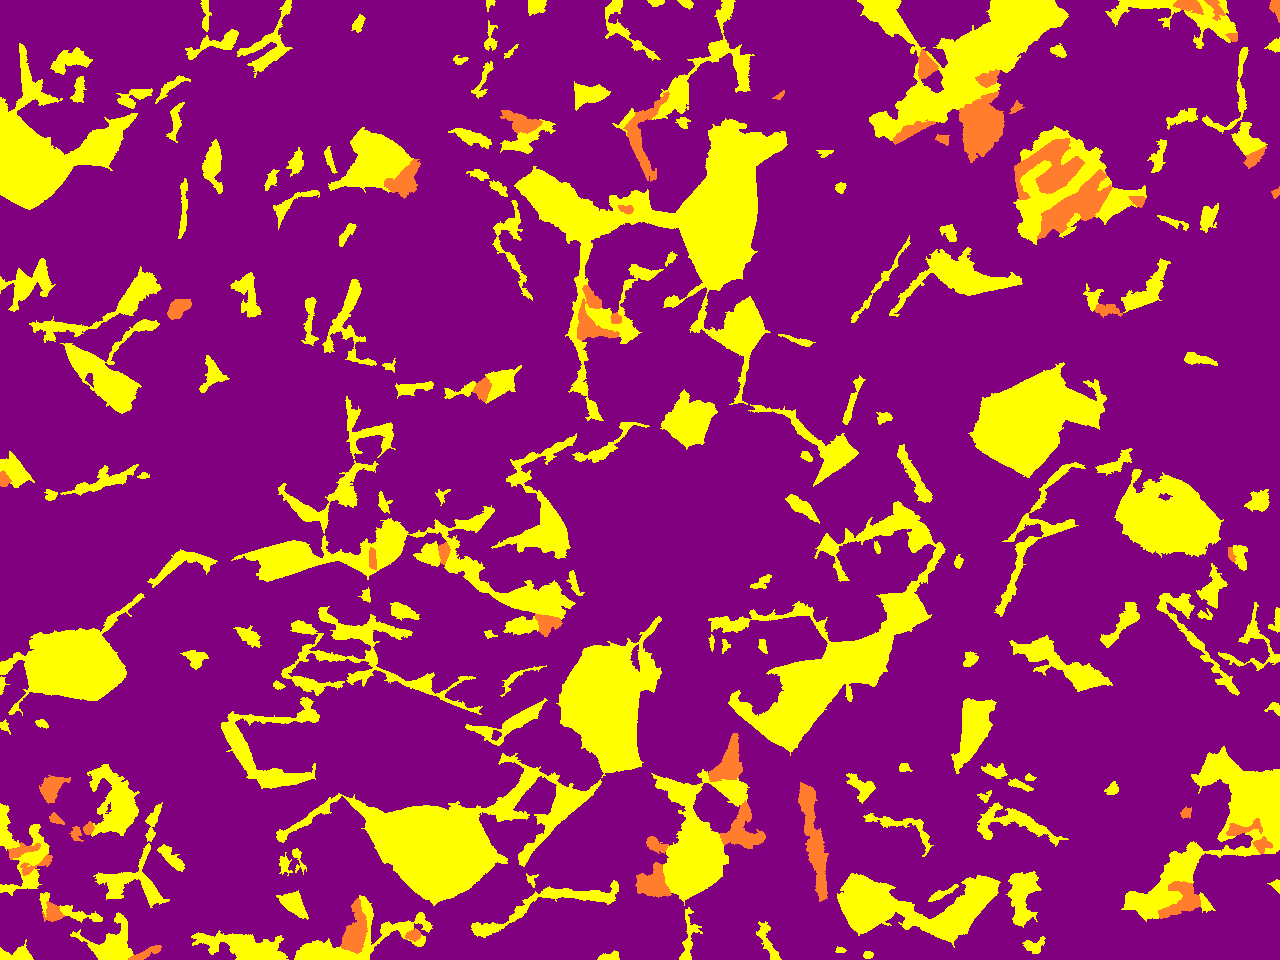
\includegraphics[width=\textwidth]{images/D3-type/1_label.png}
		\caption{D3-type label}
		\label{fig:image2.4.2}
	\end{subfigure}
	
	\begin{subfigure}[b]{0.2\textwidth}
		\centering
		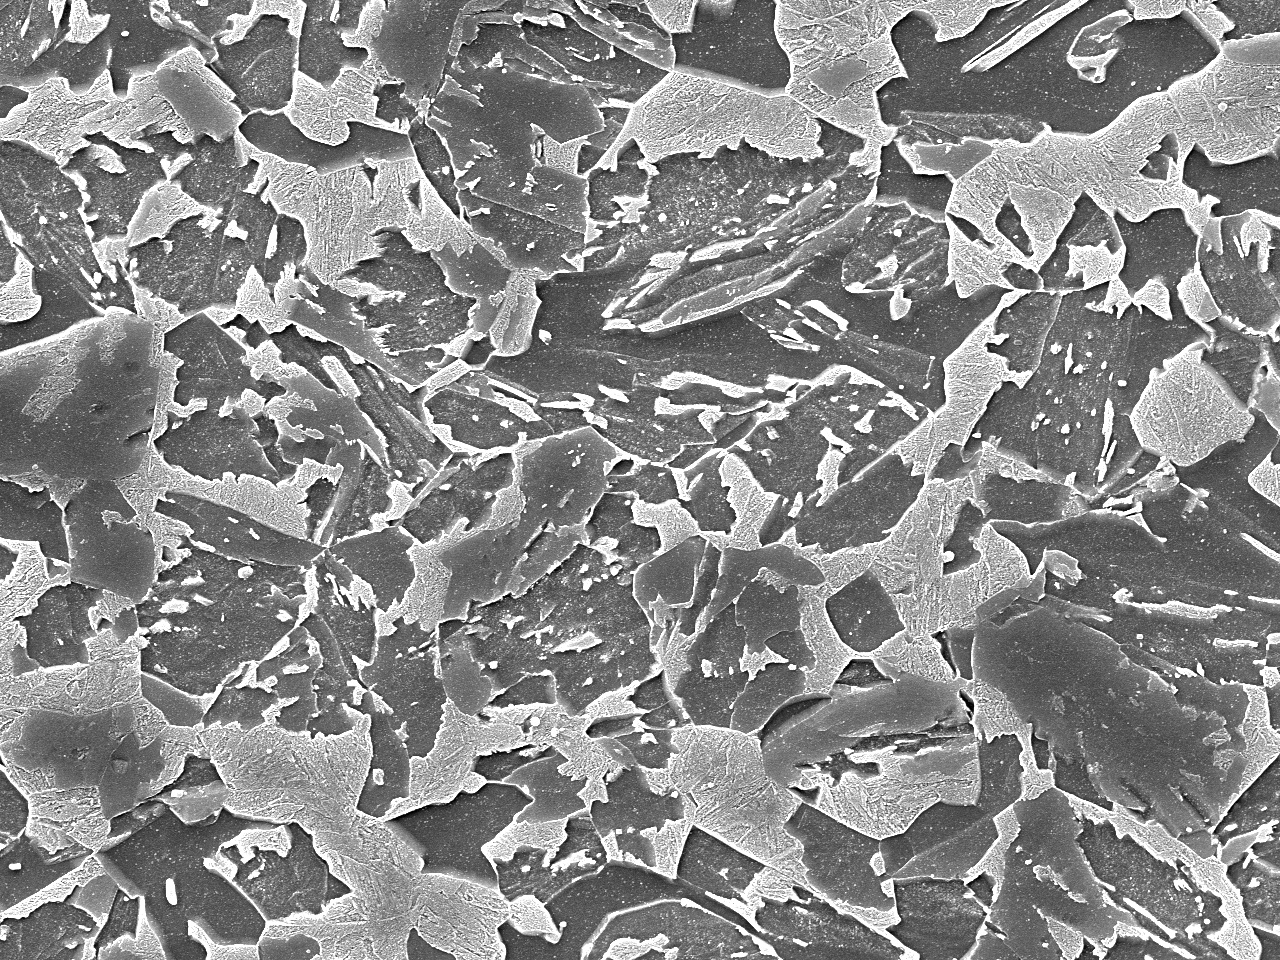
\includegraphics[width=\textwidth]{images/H2-type/1.png}
		\caption{H2-type SEM}
		\label{fig:image2.5.1}
	\end{subfigure}
	\begin{subfigure}[b]{0.2\textwidth}
		\centering
		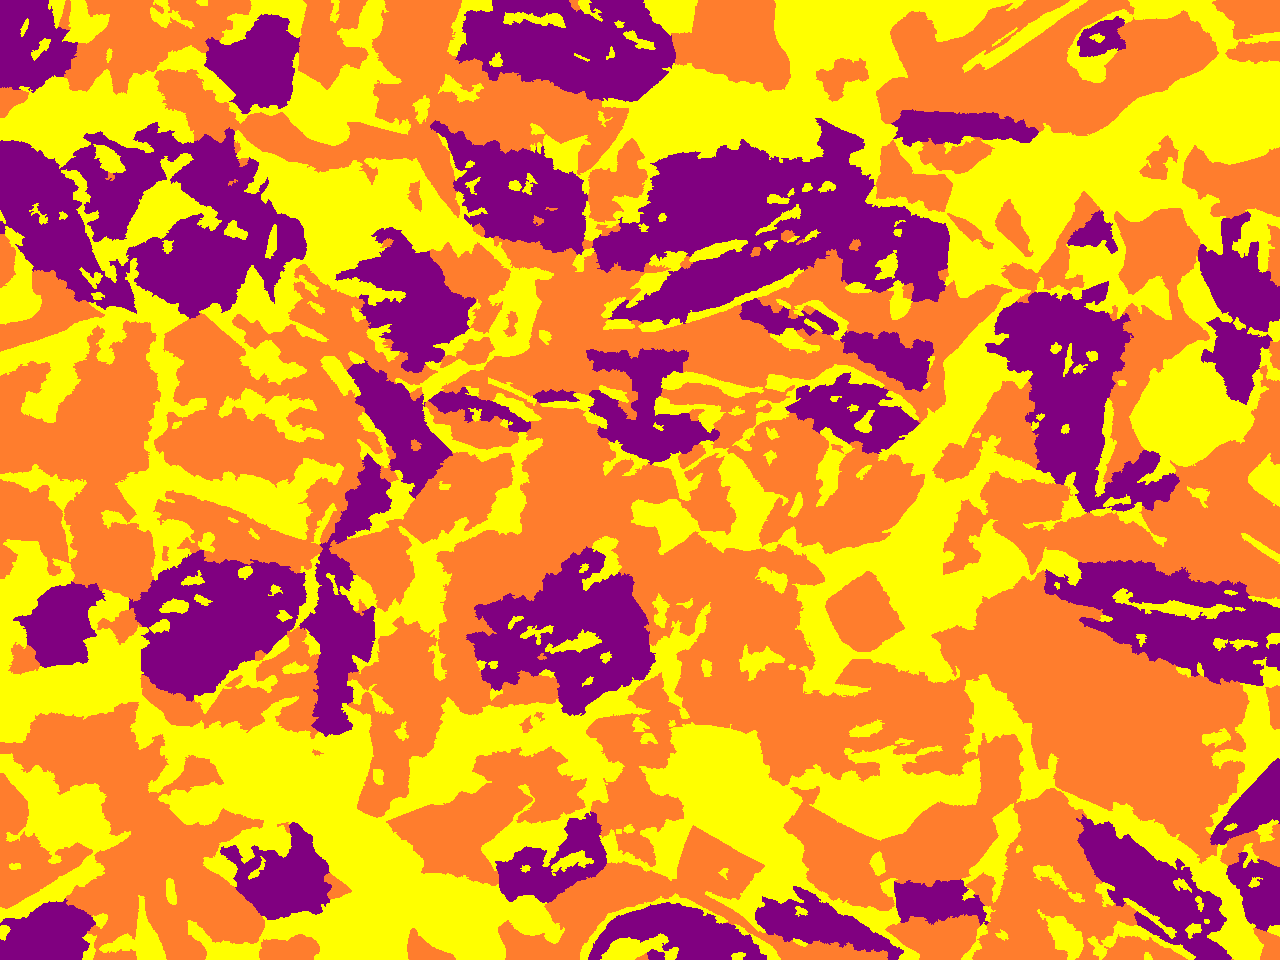
\includegraphics[width=\textwidth]{images/H2-type/1_label.png}
		\caption{H2-type label}
		\label{fig:image2.5.2}
	\end{subfigure}
	\caption{Sample images of various steel and magnification types used during inference.}
	\label{fig:combined}
\end{figure}

It's worth emphasizing that the images magnified at 3000x and 5000x originate from the same E-type steel that was used to train our model. This inclusion demonstrates the model's capacity to effectively scale across varied magnification levels, maintaining its segmentation accuracy even at high magnifications that reveal more intricate microstructures.

Furthermore, the incorporation of A-type, D3-type, and H2-type steel images, all magnified at 5000x, underscores the model's capability to generalize across different steel types. Despite these steel types featuring distinct microstructural characteristics compared to the E-type steel used in training, the model is able to accurately identify and segment their microstructures. This ability to generalize over various steel types suggests the model's potential for broad applicability in real-world industrial contexts, well beyond its initial training data.

\section{Methodology}
In the following section, we detail the methodology used in our study, which is designed to address the challenges associated with the segmentation of steel microstructures. The core of our approach involves three key components: the model architecture, the augmentation strategies, and the training process.

\subsection{Underlying U-Net Model: Design and Functionality}

The backbone of our proposed segmentation model is the U-Net architecture, a widely favored choice for image segmentation tasks. It owes its success to its ability to meticulously capture fine-grained details and preserve spatial information, which is essential in the context of steel microstructure segmentation. 

The U-Net architecture, as shown in Fig. 3, is designed as an amalgamation of an encoder path and a decoder path. The encoder path is responsible for extracting contextual information, while the decoder path contributes to accurate localization.


\begin{figure}[ht]
	\centering
	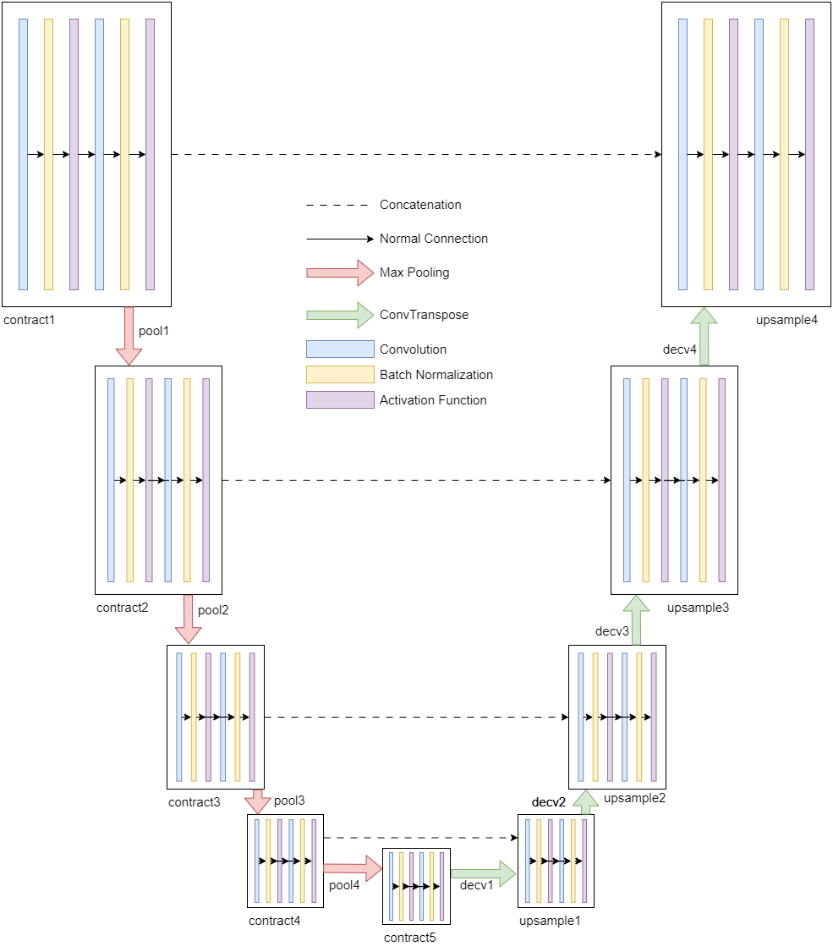
\includegraphics[width=0.7\textwidth]{images/Unet.png}
	\caption{UNet architecture}
	\label{fig:imageModel}
\end{figure}


The encoder pathway is initiated with a contraction module (contract1), dedicated to applying a series of convolutional operations to discern low-level features from the input image. Subsequent modules, identified as pool1 through pool4, carry out pooling operations that systematically reduce the spatial dimensions of the feature maps, while simultaneously augmenting the number of channels. The subsequent contraction modules, identified as contract2 through contract5, perform additional convolutional operations to distill higher-level features.

Transitioning into the decoder pathway, the architecture aims to restore spatial information and refine the segmentation outcome. The first decoder module, designated as decv1, executes convolution transpose or pixel shuffling operations, hinging on the specified anti-aliasing type. This operation is followed by an up-sampling operation (upsample1) and a concatenation procedure, amalgamating features from the equivalent layer of the encoder path. This process is reiterated through the successive decoder modules, identified as decv2 through decv4, to further enhance the feature refinement.

The final module in the decoder pathway (decv5) applies a convolutional operation to align the extracted features with the desired output classes. The activation functions integrated into the model architecture, namely sigmoid, ReLU, leaky ReLU, and swish, introduce non-linearity, thereby facilitating superior feature representation. 

The U-Net model operates under supervised learning principles. The training process leverages pixel-wise labeled images as the ground truth, optimizing the model to minimize the loss between the predicted segmentation and these labels. By utilizing the U-Net architecture, the proposed model is proficient at capturing the complex details within the microstructure of steel images and accurately segmenting various regions of interest. The synergistic combination of contraction and expansion modules enables the model to learn global contextual information as well as local, fine-grained details, culminating in precise segmentation outcomes.

\subsection{Data Augmentation Techniques and Rationale}

Data augmentation techniques serve as essential tools in confronting the issue of data insufficiency by fabricating an expanded training set through various transformations and adaptations of existing samples. In our study, we employed several augmentation techniques which not only enhanced the diversity of our training dataset but also improved our model's ability to generalize and accurately identify different microstructures. Below, we enumerate and provide a rationale for each technique employed:

\begin{itemize}
	\item Flip (x, y): We introduced horizontal (x-axis) and vertical (y-axis) flipping transformations to our images, creating mirror-like variations. This technique is beneficial as it accounts for varied orientations of steel structures, thereby ensuring our model learns to detect structures irrespective of their orientation.
	\item Rotation (0-90 degrees): Our augmentation suite includes random rotations of images within a 0 to 90-degree range. Given that steel structures in SEM images can exist in myriad orientations, this technique serves to imbue our model with rotation invariance, enabling better generalization.
	\item Zoom (1-2.5x): We applied random scaling to our images, ranging from 1 to 2.5 times their original size. This technique mimics the varied magnification levels in SEM images, thus preparing the model to handle different scales of steel structures.
	\item Intensity (0-10): We incorporated random intensity fluctuations in our images, introducing variations in brightness and darkness akin to diverse lighting conditions or material properties. This helps the model to better withstand intensity variations within steel images.
	\item Gamma (0-10): Adjusting the gamma value of our images served to enhance or suppress specific intensity levels. Gamma augmentation emulates contrast and brightness changes, thereby training the model to recognize features invariant to these differences.
	\item Contrast (HE): By applying histogram equalization (HE) to enhance image contrast, we redistributed pixel intensities to bolster overall contrast. This proved to be particularly beneficial in highlighting finer details and improving segmentation accuracy in low-contrast areas.
	\item Sliding Window: We incorporated the sliding window technique, dividing the larger input images into smaller patches of size 800x800 pixels with a stride of 15 pixels. Opting for larger patches facilitated the capture of complete structural elements, which would have been potentially obscured in smaller patches.
\end{itemize}

The integration of these augmentation techniques resulted in a model that exhibits robustness to varied orientations, scales, and contrast variations of steel microstructures. The combination of these methods resulted in an enhanced training dataset and ultimately, an improvement in the model's performance in accurately segmenting steel structures in SEM images.

\subsection{Learning Process and Parameter Settings}

Our training process was comprehensive, encompassing a range of parameter settings, optimization methodologies, and loss functions, all aimed at optimizing our model's segmentation performance. The key components of our process are enumerated below:

\begin{itemize}
	\item Optimization and Parameter Settings: We employed the Adam optimizer, renowned for its adaptive learning rate efficiency [24]. The kernel size for the convolutional layers was set to 3, allowing for effective capture of local information. We selected a batch size of 16, which proved optimal for balancing memory utilization and training efficiency. The learning rate, set at 0.00001, ensured small step sizes for smoother convergence during training. This value was carefully chosen after a series of experiments and fine-tuning to achieve optimal performance.
	\item Loss Functions: We conducted experiments with two loss functions: focal loss and Jaccard loss. Focal loss, with its emphasis on challenging samples, served to direct the model's focus towards hard-to-segment regions, while Jaccard loss or intersection-over-union (IoU) loss, measured the similarity between the predicted and ground truth masks, thereby promoting accurate segmentation. The Jaccard loss produced better results and detailed comparison between the losses in mentioned in the ablation studies section.
	\item Activation Functions: Our training process involved exploring various activation functions. Although we initially incorporated the Sinusoidal Representation Networks (Siren) activation function, our comparative analysis with the Rectified Linear Unit (ReLU) activation function revealed superior performance with ReLU. Further experiments with leaky ReLU and Swish activation functions were conducted to assess performance variations and is noted in the ablation for further reading.
	\item Experimental Techniques: To further optimize our model, we integrated blur pooling layers into the architecture and tested three variations: up, down, and both up and down. Blur pooling aids in reducing the spatial resolution of feature maps while preserving critical information, potentially enabling the model to identify larger-scale patterns and mitigate overfitting \cite{blurPooling}. Moreover, we attempted to add a boundary class to the labels by delineating edges between classes, as demonstrated in Figure 4. This approach aimed to enhance the model's ability to accurately segment the boundaries of steel structures, a critical element in proper classification and analysis. Despite the potential advantages, our experiments with blur pooling layers and the boundary class addition did not yield significant improvements in the model's performance. Detailed tabular comparisons are drawn out in the ablation studies for further reading.
	
\end{itemize}

Through the systematic exploration of different parameter settings, optimization methods, loss functions, activation functions, pooling techniques, and label modifications, our objective was to identify the most effective combination of these factors to achieve the most accurate and reliable steel image segmentation results.

\section{Experimentation}
\subsection{Evaluation Metrics}

To assess the robustness and accuracy of the proposed model, four primary metrics were used: Mean Pixel Accuracy, Dice Score, Class-wise Accuracy, and Class Distribution Ratio.

\begin{itemize}
	\item \textbf{Mean Pixel Accuracy (MPA):} This metric evaluates the pixel-level accuracy of predictions. The formula for calculating Mean Pixel Accuracy is given as:
	
	\[ MPA = \frac{1}{n_{cl}} \sum_{i} \frac{n_{ii}}{t_i} \]
	
	Here, $n_{ij}$ is the number of pixels of class $i$ predicted as class $j$, $n_{cl}$ is the total number of different classes, and $t_{i}$ is the sum of all pixels of class $i$ ($t_{i} = \sum_{j} n_{ij}$).
	
	\item \textbf{Dice Score (F1 Score):} The Dice Score computes the overlap between the predicted segmentation mask (A) and the ground truth mask (B). The formula is:
	
	\[ Dice = \frac{2 |A \cap B|}{|A| + |B|} \]
	
	Here, $A$ is the predicted segmentation mask, $B$ is the ground truth mask, $|A|$ is the number of pixels in $A$, $|B|$ is the number of pixels in $B$, $|A \cap B|$ calculates the intersection of $A$ and $B$.
	
	\item \textbf{Class-wise Accuracy:} This metric measures the accuracy of model's predictions for each individual class, providing a detailed understanding of its performance across different classes.
	
	\item \textbf{Class Distribution Ratio:} This metric compares the distribution of classes in the predicted segmentation masks with the distribution in the ground truth labels, to identify any potential biases or imbalances in the model's predictions.
\end{itemize}

These metrics holistically measure the performance of the proposed model, reflecting its ability to accurately segment various microstructures, and its generalization across different classes. Utilizing these metrics ensures a balanced and comprehensive evaluation of the model's effectiveness in predicting steel microstructures, providing a well-rounded understanding of its performance.

\subsection{Experiment Setup}

Our model's experimental setup is designed to train and evaluate the model using a combination of different steel images and testing methodologies. The setup uses a high-performance computing system equipped with an NVIDIA A6000 GPU, Intel i7 6700 CPU, running on the Ubuntu 22.10 operating system, and utilizing the PyTorch framework.

\begin{itemize}
	\item \textbf{Data Preparation:} To create an effective training dataset, five out of six available images were chosen for augmentation. The remaining image was reserved solely for testing. This strategy provided a sufficient amount of data for training while also ensuring an independent dataset for testing the model's generalization performance. The color-coding of the label images was converted into class labels: purple (Bainite) was denoted as 0, orange (Ferrite) as 1, and yellow (Martensite) as 2.
	
	\item \textbf{Training and Validation Split:} The augmented dataset was further partitioned into a training set and a validation set with a split ratio of 0.8. This meant 80\% of the augmented images were used for model training, while the remaining 20\% were used for validation. This approach facilitated performance monitoring and model fine-tuning during the training process.
	
	\item \textbf{Model Testing:} Post-training, the model was tested on an image not used during the training or augmentation process. This unseen data served to evaluate the model's capacity to generalize and accurately segment the steel structures. Additionally, X3000, x5000, A, H2, D3 steel type images were inferenced using the saved model post-training.
\end{itemize}


\subsection{Experimental Results}

In this section, we describe the results obtained from the experimental setup. We categorize the inference scenarios into three main categories: inferencing with the same steel type and magnification as the trained model, inferencing with the same steel type but different magnification levels, and inferencing with different steel types and different magnification levels compared to the trained model. 

\subsubsection{Inference on Same Steel and Same Magnification}

The trained model was evaluated using a test image that was isolated from the training process. The model achieved an overall accuracy of 91.74\%, with a mean Intersection over Union (mIoU) of 0.46825. The class-wise accuracy analysis showed that the model performed significantly well across different classes: Martensite (83.7\%), Ferrite (96.1\%), and Bainite (81.3\%).


\begin{figure}[ht]
	\centering
	
	\begin{subfigure}[b]{0.3\textwidth}
		\centering
		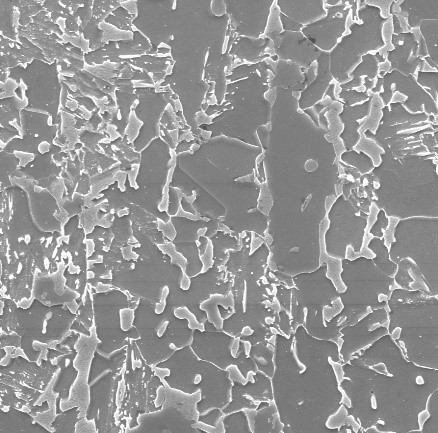
\includegraphics[width=\textwidth]{images/inference/SameSteelSameMag-O.jpg}
		\caption{}
		\label{fig:samesteelsamemag-orig}
	\end{subfigure}
	\hfill
	\begin{subfigure}[b]{0.3\textwidth}
		\centering
		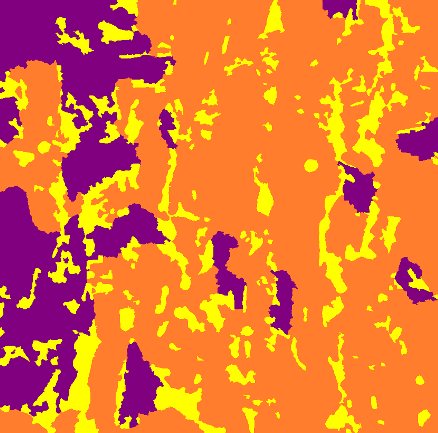
\includegraphics[width=\textwidth]{images/inference/SameSteelSameMag-L.png}
		\caption{}
		\label{fig:samesteelsamemag-label}
	\end{subfigure}
	\hfill
	\begin{subfigure}[b]{0.3\textwidth}
		\centering
		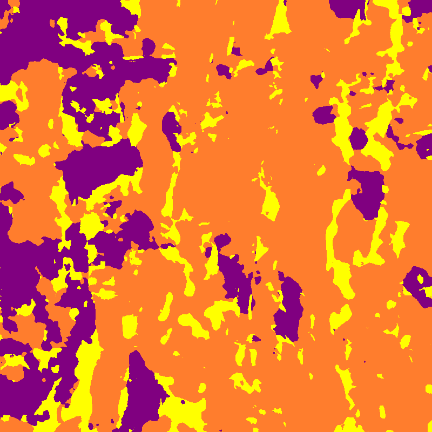
\includegraphics[width=\textwidth]{images/inference/SameSteelSameMag-P.png}
		\caption{}
		\label{fig:samesteelsamemag-pred}
	\end{subfigure}
	
	\caption{(a) x2700 magnified E type SEM test image (b) Corresponding label image by EBSD (c) Image predicted by our model.}
	\label{fig:samesteelsamemag}
\end{figure}



\begin{table}[h!]
	\centering
	\begin{tabular}{|c|c|}
		\hline
		\textbf{Image Type} & \textbf{Test Image Accuracy}\\
		\hline
		Accuracy & 91.74 (0.9158) \\
		\hline
		Martensite & 83.7 \\
		Ferrite & 96.1 \\
		Bainite & 81.3 \\
		\hline
	\end{tabular}
	\caption{Accuracy and Dice measurements of test image}
\end{table}

\subsubsection{Inference on Same Steel with Different Magnification}

Images of the same Steel type (E type) but at different magnification levels were used for inference. Images at x3000 and x5000 zoom levels were used, revealing accuracies of 84.11\% and 89.3\%, respectively. The additional evaluation metrics, including the Dice score, accuracy per class, and class ratio, provided a deeper understanding of the model performance across different magnification levels. 
\begin{figure}[ht]
	\centering
	
	\begin{subfigure}[b]{0.3\textwidth}
		\centering
		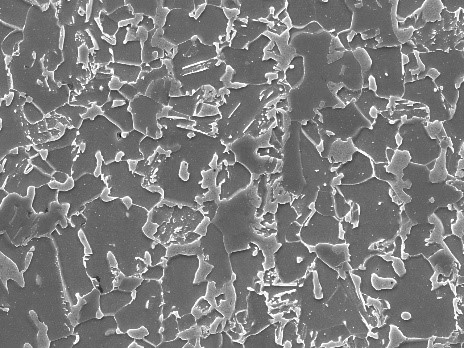
\includegraphics[width=\textwidth]{images/inference/SameSteelDiffMag-O.jpg}
		\caption{}
		\label{fig:samesteeldiffmag3K-orig}
	\end{subfigure}
	\hfill
	\begin{subfigure}[b]{0.3\textwidth}
		\centering
		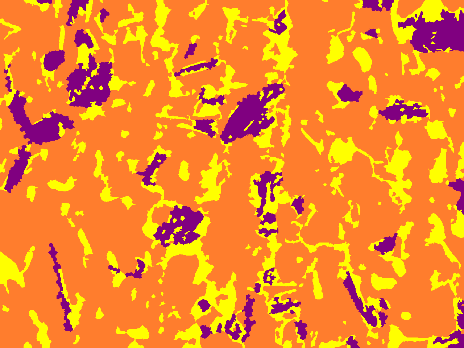
\includegraphics[width=\textwidth]{images/inference/SameSteelDiffMag-L.png}
		\caption{}
		\label{fig:samesteeldiffmag3K-label}
	\end{subfigure}
	\hfill
	\begin{subfigure}[b]{0.3\textwidth}
		\centering
		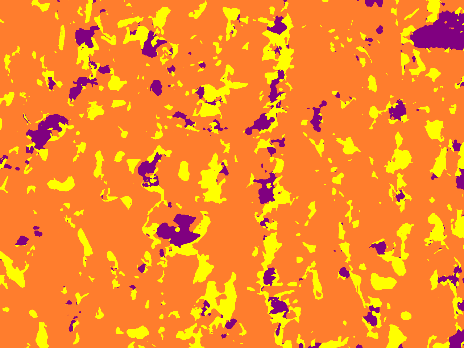
\includegraphics[width=\textwidth]{images/inference/SameSteelDiffMag-P.png}
		\caption{}
		\label{fig:samesteeldiffmag3K-pred}
	\end{subfigure}
		\begin{subfigure}[b]{0.3\textwidth}
		\centering
		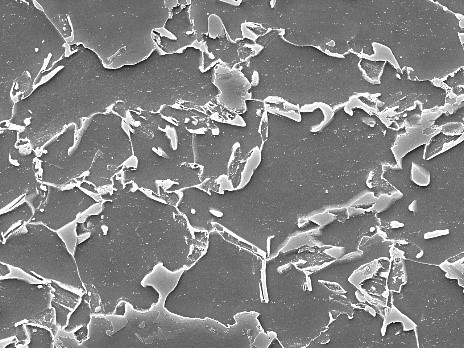
\includegraphics[width=\textwidth]{images/inference/SameSteelDiffMag-2-O.jpg}
		\caption{}
		\label{fig:samesteeldiffmag5K-orig}
	\end{subfigure}
	\hfill
	\begin{subfigure}[b]{0.3\textwidth}
		\centering
		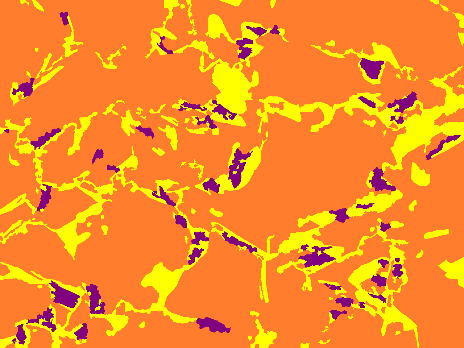
\includegraphics[width=\textwidth]{images/inference/SameSteelDiffMag-2-L.png}
		\caption{}
		\label{fig:samesteeldiffmag5K-label}
	\end{subfigure}
	\hfill
	\begin{subfigure}[b]{0.3\textwidth}
		\centering
		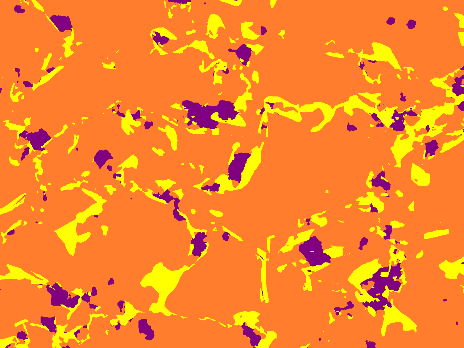
\includegraphics[width=\textwidth]{images/inference/SameSteelDiffMag-2-P.png}
		\caption{}
		\label{fig:samesteeldiffmag5K-pred}
	\end{subfigure}
	
	\caption{(a), (b) x3000 magnified E type SEM test image and corresponding label; (d), (e) x5000 magnified E type SEM test image and corresponding label; (c), (f) Images predicted by our model.}
	\label{fig:samesteeldiffmag}
\end{figure}


\begin{table}[h!]
	\centering
	\begin{tabular}{|c|c|c|}
		\hline
		\textbf{Metrics} & \textbf{X3000 E Type} & \textbf{X5000 E Type}\\
		\hline
		Accuracy & 84.11 & 89.29 \\
		\hline
		Dice Score & 0.8377 & 0.8852 \\
		\hline
		Accuracy Per Class & 68.11, 93.77, 45.33 & 70.87, 96.57, 41.73 \\
		\hline
		Class Ratio [label] & 0.1982, 0.7029, 0.0989 & 0.176, 0.7789, 0.0451 \\
		\hline
		Class Ratio [Predicted] & 0.1514, 0.7904, 0.0583 & 0.1282, 0.8196, 0.0522 \\
		\hline
		Error Margin of Class Ratio & -0.0438, +0.0875, -0.0406 & -0.0478, +0.0407, +0.0071 \\
		\hline
	\end{tabular}
	\caption{Different metrics of predicted images of x3000 and x5000 E type steel}
\end{table}

\subsubsection{Inference on Different Steel and Different Magnification}

The performance of the model was further assessed on images of different steel types and magnification levels not included in the training data. The model demonstrated decent accuracies on these images, with A type steel images achieving 74.78\%, D3 type achieving 68.3\%, and H2 type achieving nearly 74\%. 


\begin{figure}[!h]
	\centering
	
	\begin{subfigure}[b]{0.3\textwidth}
		\centering
		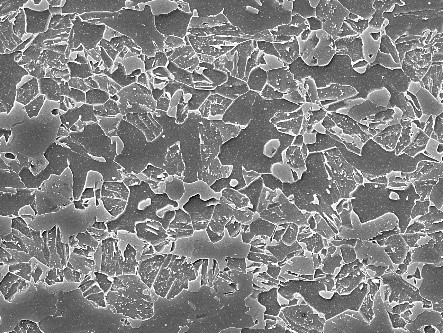
\includegraphics[width=\textwidth]{images/inference/A-type-O.jpg}
		\caption{}
		\label{fig:A-type-orig}
	\end{subfigure}
	\hfill
	\begin{subfigure}[b]{0.3\textwidth}
		\centering
		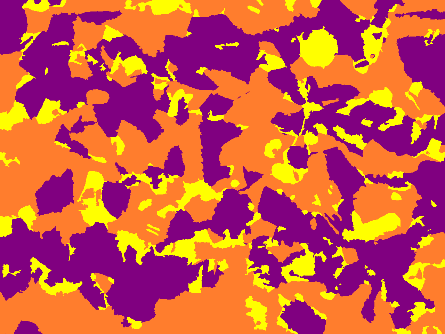
\includegraphics[width=\textwidth]{images/inference/A-type-L.png}
		\caption{}
		\label{fig:A-type-label}
	\end{subfigure}
	\hfill
	\begin{subfigure}[b]{0.3\textwidth}
		\centering
		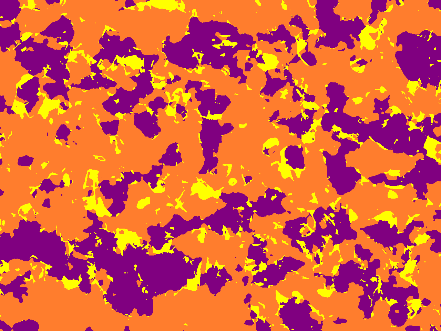
\includegraphics[width=\textwidth]{images/inference/A-type-P.png}
		\caption{}
		\label{fig:A-type-pred}
	\end{subfigure}
	\begin{subfigure}[b]{0.3\textwidth}
		\centering
		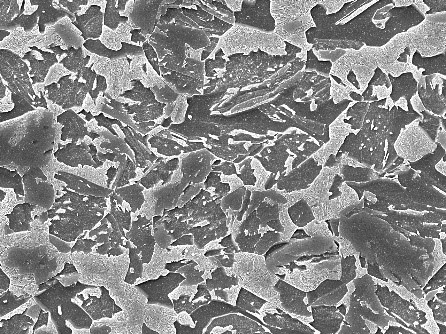
\includegraphics[width=\textwidth]{images/inference/H2-type-O.jpg}
		\caption{}
		\label{fig:H2-type-orig}
	\end{subfigure}
	\hfill
	\begin{subfigure}[b]{0.3\textwidth}
		\centering
		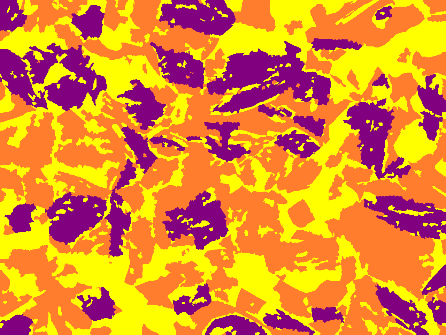
\includegraphics[width=\textwidth]{images/inference/H2-type-L.png}
		\caption{}
		\label{fig:H2-type-label}
	\end{subfigure}
	\hfill
	\begin{subfigure}[b]{0.3\textwidth}
		\centering
		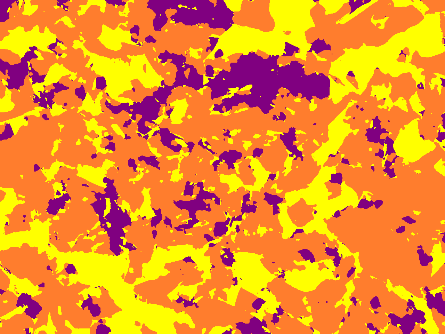
\includegraphics[width=\textwidth]{images/inference/H2-type-P.png}
		\caption{}
		\label{fig:H2-type-pred}
	\end{subfigure}
	\begin{subfigure}[b]{0.3\textwidth}
		\centering
		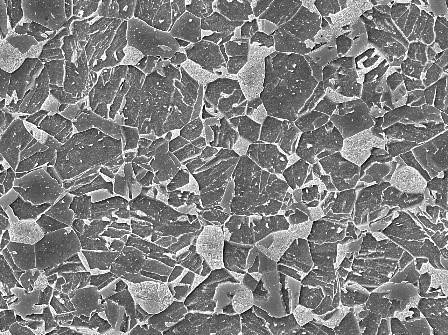
\includegraphics[width=\textwidth]{images/inference/D3-type-O.jpg}
		\caption{}
		\label{fig:D3-type-orig}
	\end{subfigure}
	\hfill
	\begin{subfigure}[b]{0.3\textwidth}
		\centering
		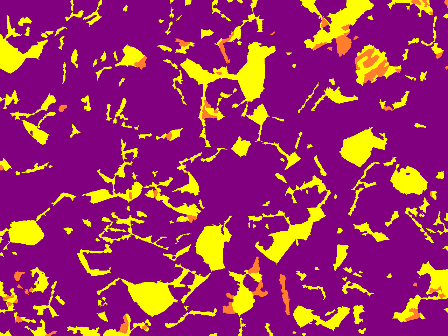
\includegraphics[width=\textwidth]{images/inference/D3-type-L.png}
		\caption{}
		\label{fig:D3-type-label}
	\end{subfigure}
	\hfill
	\begin{subfigure}[b]{0.3\textwidth}
		\centering
		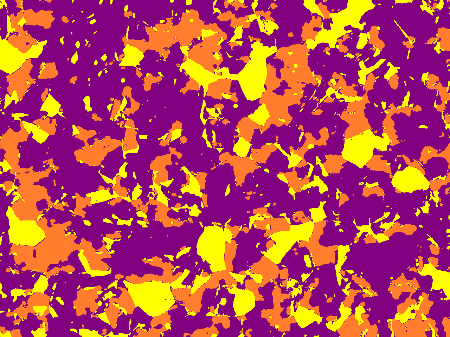
\includegraphics[width=\textwidth]{images/inference/D3-type-P.png}
		\caption{}
		\label{fig:D3-type-pred}
	\end{subfigure}
	
	\caption{(a), (b) x5000 magnified A type SEM test image and corresponding label; (d), (e) x5000 magnified D3 type SEM test image and corresponding label; (g), (h) x5000 magnified H2 type SEM test image and corresponding label; (c), (f) and(i) Images predicted by our model.}
	\label{fig:diffsteeldiffmag}
\end{figure}


\begin{table}[h!]
	\centering
	\begin{tabular}{|c|c|c|c|}
		\hline
		\textbf{Metrics} & \textbf{A type} & \textbf{D3 Type} & \textbf{H2 Type}\\
		\hline
		Pixel Accuracy & 74.78 & 68.32 & 73.89 \\
		\hline
		Dice Score & 0.7365 & 0.6791 & 0.7248 \\
		\hline
		Accuracy Per Class & 51.04, 92.11, 65.45 & 79.64, 24.41, 66.89 & 78.52, 88.11, 37.62 \\
		\hline
		Class Ratio [label] & 0.1441, 0.4281, 0.4278 & 0.1742, 0.0184, 0.8074 & 0.3404, 0.4313, 0.2283 \\
		\hline
		Class Ratio [Predicted] & 0.1, 0.5683, 0.3317 & 0.1796, 0.236, 0.5844 & 0.2819, 0.573, 0.1451 \\
		\hline
		Error Margin of Class Ratio & -0.0441, 0.1402, -0.0961 & 0.0054, 0.2176, -0.223 & -0.0585, 0.1417, -0.0832 \\
		\hline
	\end{tabular}
	\caption{Different metrics of predicted images of different types of steel}
\end{table}

\subsection{Ablation Studies}

\subsubsection{Activation Function}
Different activation functions were examined to determine their impact on the model performance. While Siren activation functions are known for capturing complex patterns and functions, in this specific task of steel image segmentation, ReLU performed better as illustrated in Table 2.

\begin{table}[h!]
	\centering
	\begin{tabular}{|c|c|c|c|c|c|}
		\hline
		Activation & X3000 E Type & X5000 E Type & A Type & D3 Type & H2 Type \\
		\hline
		Siren & 86.12 (0.8487) & 89.77 (0.8853) & 74.87 (0.7383) & 40.02 (0.3994) & 69.8 (0.6855) \\
		\rowcolor{yellow!30} ReLU & 83.97 (0.8272) & 90.01 (0.8976) & 77.41 (0.7716) & 64.75 (0.6397) & 73.89 (0.7364) \\
		Leaky ReLU & 84.77 (0.8452) & 88.53 (0.8831) & 75.19 (0.7493) & 59.59 (0.5855) & 69.69 (0.6938) \\
		Swish & 84.21 (0.8396) & 88.67 (0.8842) & 72.41 (0.7217) & 56.54 (0.5649) & 70.00 (0.6973) \\
		\hline
	\end{tabular}
	\caption{Accuracy and dice measurements along with class-wise accuracy for models with different activation functions.}
\end{table}

\subsubsection{Effects of Blur Pooling}
Blur pooling layers were tested in different combinations to analyze their impact on model performance. As observed, blur pooling combined with Siren activation function showed improvements, however, with ReLU it performed poorly.

\begin{table}[h!]
	\centering
	\begin{tabular}{|c|c|c|c|c|c|}
		\hline
		Blur Pool & X3000 E Type & X5000 E Type & A Type & D3 Type & H2 Type \\
		\hline
		\rowcolor{yellow!30} None & 83.97 (0.8272) & 90.01 (0.8976) & 77.41 (0.7716) & 64.75 (0.6397) & 73.89 (0.7364) \\
		Down & 83.53 (0.8329) & 87.69 (0.8743) & 70.83 (0.7061) & 52.5 (0.5227) & 68.02 (0.6777) \\
		Up & 84.41 (0.8416) & 87.93 (0.8768) & 76.73 (0.7648) & 45.04 (0.4479) & 69.0 (0.6875) \\
		Down + Up & 84.3 (0.8405) & 87.51 (0.8726) & 74.5 (0.7425) & 40.24 (0.3999) & 66.78 (0.6653) \\
		\hline
	\end{tabular}
	\caption{Accuracy and dice measurements along with class-wise accuracy for models with different Blur pooling layers.}
\end{table}

\subsubsection{Loss Functions}
We experimented with two loss functions, Focal Loss and Jaccard Loss. Jaccard Loss performed marginally better than Focal Loss as it directly penalizes false positives and false negatives, making it suitable for image segmentation tasks.

\begin{table}[h!]
	\centering
	\begin{tabular}{|c|c|c|c|c|c|}
		\hline
		Loss & X3000 E Type & X5000 E Type & A Type & D3 Type & H2 Type \\
		\hline
		Focal & 83.97 (0.8272) & 90.01 (0.8976) & 77.41 (0.7716) & 64.75 (0.6397) & 73.89 (0.7364) \\
		\rowcolor{yellow!30} Jaccard & 84.11 (0.8389) & 89.29 (0.8892) & 77.78 (0.7731) & 68.32 (0.6809) & 73.92 (0.7376) \\
		\hline
	\end{tabular}
	\caption{Accuracy and dice measurements along with class-wise accuracy for models with different loss functions.}
\end{table}

\subsubsection{Classification with Boundary Class}
Introducing a boundary class in the classification task was intended to improve boundary localization, enhancing discrimination, reducing ambiguity, and enabling fine-grained analysis.

\begin{table}[h!]
	\centering
	\begin{tabular}{|c|c|c|c|c|c|}
		\hline
		Class & X3000 E Type & X5000 E Type & A Type & D3 Type & H2 Type \\
		\hline
		\rowcolor{yellow!30} No Boundary Class & 84.11 (0.8389) & 89.29 (0.8892) & 77.78 (0.7731) & 68.32 (0.6809) & 73.92 (0.7376) \\
		Boundary Class & 80.04 (0.7979) & 84.94 (0.8469) & 70.95 (0.707) & 62.53 (0.6228) & 65.02 (0.6477) \\
		\hline
	\end{tabular}
	\caption{Accuracy and dice measurements along with class-wise accuracy for models with boundary class and non-boundary class.}
\end{table}



\section{Discussion}

The experimental results from this study provide valuable insights into the nuances of steel image segmentation. This section provides an analysis and interpretation of these results, addressing the strengths and limitations of our approach, investigating the factors influencing performance variations, discussing the encountered challenges, and outlining potential future work and improvement areas.

\subsection{Experimental Results Analysis and Interpretation}

In this study, we evaluated different aspects of the model, including activation functions, blur pooling, loss functions, and the incorporation of a boundary class. Contrary to initial expectations, the results showed that the Rectified Linear Unit (ReLU) activation function outperformed the SIREN, LeakyReLU, and Swish activation functions. 

Blur Pooling showed promising results when coupled with the SIREN activation function, yet it fell short when paired with ReLU. Jaccard Loss notably outperformed Focal Loss in terms of accuracy and segmentation performance. Interestingly, the inclusion of a boundary class did not significantly improve the segmentation results. The comparison of these varying methodologies revealed that the optimal combination for accurate steel image segmentation is the ReLU activation function and Jaccard loss. The experiment results are detailed in the the ablation studies section.

\subsection{Challenges and Limitations}

A major challenge encountered in this study is the limited amount of training data. With just six images, the training dataset might not sufficiently capture the diversity and complexity of real-world steel images, potentially affecting the model's generalization capabilities. 

Additionally, there are instances where a microstructure in the steel images may appear similar yet have different compositions. It is a complex task for the model to identify such intricate details in the images, representing another limitation in our current approach.

\subsection{Factors Contributing to Performance Variations}

Several factors contribute to the observed performance variations. Primarily, the choice of activation function significantly impacted the model's ability to capture relevant features for accurate segmentation. 

Moreover, the interplay between activation functions and blur pooling highlights the importance of their compatibility, reinforcing that optimal results are dependent on their combination rather than individual merits. 

The choice of loss function played a critical role in effectively guiding the model's learning process and achieving accurate segmentation results. 

Interestingly, the incorporation of a boundary class did not yield significant improvements, suggesting that boundary information alone might not suffice for enhancing segmentation performance. 


\section{Conclusion}

The challenge of accurate microstructure segmentation in metallographic images has been addressed in this research using a deep learning-based approach. Through a series of comprehensive experiments and in-depth analyses, several crucial findings and contributions have emerged. 

A detailed investigation into different aspects of the proposed model, including activation functions, loss functions, and the impact of blur pooling, revealed that the Rectified Linear Unit (ReLU) activation function combined with Jaccard loss provided the best results. Interestingly, while blur pooling showed potential improvements when paired with certain activation functions, it exhibited suboptimal performance with ReLU.

To assess the generalization capabilities of our model, we conducted inference on a variety of images. The model demonstrated impressive accuracy on images with the same steel type and magnification levels as those used during training. It also showed strong performance on images of the same steel type but different magnification levels. Importantly, the model maintained decent accuracy even when confronted with images of different steel types and magnification levels, exhibiting a robust ability to generalize.

The ability to accurately segment microstructures in metallographic images holds immense importance in various industrial applications, particularly in the context of quality control during steel production and materials characterization. The proposed approach has shown significant promise in addressing this task, offering an automated solution that can reduce human effort and enhance efficiency in metallographic image analysis. The effectiveness of our approach, coupled with its potential industrial applications, underscores the practical value of this research.

Accurate microstructure segmentation allows manufacturers to derive valuable insights into material properties, inform decision-making processes, and refine quality control measures. 

Looking towards the future, there is room for further research and development. Exploring the utilization of advanced architectures and techniques, such as attention mechanisms and multi-scale analysis, could potentially enhance the accuracy and robustness of the segmentation model. In addition, expanding the scope of the study to include a wider variety of steel types and investigating the influence of different imaging conditions would undoubtedly enhance the model's real-world applicability and utility.




\bibliography{reference}
\bibliographystyle{plain}
\end{document}
